
\documentclass[letterpaper]{article}
\usepackage{aaai21}
\usepackage{times}
\usepackage{helvet}
\usepackage{courier}
%\usepackage[hyphens]{url}
\usepackage{graphicx}
\usepackage{subcaption}
%\urlstyle{rm}
%\def\UrlFont{\rm}
%\usepackage{graphicx}
\frenchspacing
\setlength{\pdfpagewidth}{8.5in}
\setlength{\pdfpageheight}{11in}
\usepackage{wrapfig}

\usepackage{url}
\urlstyle{rm} % DO NOT CHANGE THIS
\def\UrlFont{\rm}  % DO NOT CHANGE THIS

%\usepackage{color}
\usepackage{color,soul}



\usepackage{todonotes}
\usepackage{multicol}

%% TODO: Check which packages unnecessary
\usepackage{pifont}
\usepackage{natbib}
\usepackage{caption}

%\usepackage{geometry}
%\usepackage{fleqn}
%\usepackage{graphicx}
\usepackage{txfonts}
%\usepackage{hyperref}
\usepackage{lineno}
\usepackage[figuresright]{rotating}

\definecolor{GreenYellow}{RGB}{210,255,92}

\newcommand\note[1]{\todo[inline, color=red!40]{#1}}
\newcommand\mNote[1]{\todo[inline, author=Michael, color=cyan]{#1}}
\newcommand\maNote[1]{\todo[inline, author=Maor, color=green]{#1}}
\newcommand\rNote[1]{\todo[inline, author=Ronen, color=yellow]{#1}}
\newcommand\aNote[1]{\todo[inline, author=Alex, color=GreenYellow]{#1}}
\newcommand\commentout[1]{}

%%%
%\newcommand{\shashank}[1]{\textbf{\color{cyan}[Shashank:#1]}}

\definecolor{frameColor}{RGB}{204,204,204}
\usepackage{xcolor}
\usepackage{float}
\usepackage{subcaption}

\newcommand{\frameImage}[4]{
\begin{figure}[H]
  \centerline{
    \fcolorbox{frameColor}{white}{
        \includegraphics[height=#2, width=#3]{#1} } }
    \caption{#4}
    \label{fig:#1}
\end{figure}
}


\definecolor{ColorNodeName}{RGB}{140, 56, 99}
\definecolor{ColorNodeInvariant}{RGB}{167, 66, 168}
\definecolor{ColorEdgeGuard}{RGB}{66, 168, 72  }
\definecolor{ColorEdgeProbability}{RGB}{168, 122, 66}
\definecolor{ColorEdgeUpdate}{RGB}{66, 66, 168}
\definecolor{ColorEdgeSynchronization}{RGB}{66, 160, 168}

\newcommand\colorsCellHeight {4}
\newcommand\colorsCellWidth  {10}

% \newcommand\colorsTable  {
% \begin{table}[]
% \centering
% \begin{tabular}{|l|c|l|c|} \hline
% \tiny Attribute               & \tiny Color
% & \tiny Attribute               & \tiny Color\\ \hline
% \tiny Node name               & \fcolorbox{ColorNodeName}{ColorNodeName}{\makebox(\colorsCellWidth,\colorsCellHeight){}}
% & \tiny Node invariant          & \fcolorbox{ColorNodeInvariant}{ColorNodeInvariant}{\makebox(\colorsCellWidth,\colorsCellHeight){}} \\ \hline
% \tiny Edge guard              & \fcolorbox{ColorEdgeGuard}{ColorEdgeGuard}{\makebox(\colorsCellWidth,\colorsCellHeight){}}
% & \tiny Edge probability        & \fcolorbox{ColorEdgeProbability}{ColorEdgeProbability}{\makebox(\colorsCellWidth,\colorsCellHeight){}} \\ \hline
% \tiny Edge update             & \fcolorbox{ColorEdgeUpdate}{ColorEdgeUpdate}{\makebox(\colorsCellWidth,\colorsCellHeight){}}
% & \tiny Edge synchronization    & \fcolorbox{ColorEdgeSynchronization}{ColorEdgeSynchronization}{\makebox(\colorsCellWidth,\colorsCellHeight){}} \\ \hline
% \end{tabular}
% %\caption{Color legend for PTA}
% \end{table}
% }

% For /Title, add Title in Mixed Case. No accents or commands. Retain the parentheses.

\setcounter{secnumdepth}{0} %May be changed to 1 or 2 if section numbers are desired.

%\setlength\titlebox{2.5in} % If your paper contains an overfull \vbox too high warning at the beginning of the document, use this
% command to correct it. You may not alter the value below 2.5 in
\title{Verifying Plans and Scripts for Robotics Tasks \\ Using Performance Level Profiles}
%Your title must be in mixed case, not sentence case.
% That means all verbs (including short verbs like be, is, using,and go),
% nouns, adverbs, adjectives should be capitalized, including both words in hyphenated terms, while
% articles, conjunctions, and prepositions are lower case unless they
% directly follow a colon or long dash

% \author{
% Alexander Kovalchuk, Shashank Shekhar {\normalfont and} Ronen I. Brafman\\
% Ben-Gurion University of the Negev, Beer Sheva, Israel\\
% \{kovalchu, shekhar, brafman\}@cs.bgu.ac.il
% }

\author{
    Alexander Kovalchuk, Shashank Shekhar {\normalfont and} Ronen I. Brafman \\
    % Department of Computer Science\\
    % Ben Gurion University\\
    % shekhar@cs.bgu.ac.il
    % \And
    % Ronen I. Brafman\\
    % Department of Computer Science\\
    % Ben Gurion University\\
    % brafman@cs.bgu.ac.il
    % \And
    % Guy Shani\\
    % Information and Software Systems Eng.\\
    % Ben Gurion University\\
    % shanigu@bgu.ac.il
}

\affiliations{
    % \textsuperscript{\rm 1}
    The Department of Computer Science \\
    %\textsuperscript{\rm 2} Information and Software Systems Engineering \\
    Ben-Gurion University of the Negev, Beer-Sheva, Israel \\
    \{kovalchu, shekhar, brafman\}@cs.bgu.ac.il %brafman@cs.bgu.ac.il,
    %shanigu@bgu.ac.il
}


% All authors must be in the same font size and format. Use \Large and \textbf to achieve this result when breaking a line
\begin{document}

\maketitle




\begin{abstract}
{\em Performance-Level Profiles (PLPs)\/} were introduced as a
type of action representation language suitable for capturing the behavior of functional code for robotics. This paper considers two issues that PLPs raise: (1) Their formal semantics. (2) How to verify a script or plans that schedule the use of components that have been documented by PLPs. We discuss formal semantics for PLPs that maps them to probabilistic timed automata (PTAs). We also show how, given a script that refers to components specified using PLPs, we derive a PTA specification of the entire system. Using a model checker, we can now verify various properties of the system and answers queries about its behavior. Finally, we empirically evaluate an implemented system based on these ideas that use the UPPAAL-SMC model checker
and demonstrate its scalability. The result is a pragmatic approach for verifying various properties of component-based robotic systems.
\end{abstract}


%%%%%%%%%%%%%%%%%%%%%%%%%%%%%%%%%%%%%%%%%%%%%%%%%%%%%%%%%%%%%%%%%%%%%%%%%%%%%%%%


\section{Introduction}
Most robotic systems are built by assembling software components, locally written, or imported, each of which handles a particular capability. A more sophisticated behavior is then obtained by combining these behaviors in various ways.
Unfortunately, as noted in~\citet{Abdellatif12}: ``Systems built by assembling together, independently developed and delivered components often exhibit pathological behavior. Part of the problem is that developers of these systems do not have {\bf a precise way of expressing the behavior of components}..."
%at their interfaces, where inconsistencies may occur."
Addressing this issue is crucial to our ability to deploy autonomous robots in open environments.

%Lacking a precise definition of normal behavior, how will we identify abnormal one? Certainly, we would not want to wait until
%%the last moment where
%some evidently undesirable outcome occurs, nor is the public likely to tolerate such performance. Moreover, even before deployment, users would want to understand what they are getting before spending large amounts of money and/or time on an autonomous robot, or using some package.

%To some extent, we can address these issues by providing good code documentation.
\citet{PLP-IROS16} advocated the use of an intuitive {\em machine readable\/} descriptive (rather than normative, or prescriptive) behavior specifications. Such specifications make more precise what must be said and how,
and they enable the development of tools that can utilize them to {\em automatically\/} support monitoring, validation, and planning.
%Unfortunately, functional modules without clear formal semantics are difficult to combinen novel ways, as would befit an autonomous robot, which is offered by more principled formal tools.
%Given this state of affairs, if robotic infrastructure is to reach a plug-and-play state, as in personal computing, we must be able to combine diverse robotic modules and components easily, and automatically. Yet,
%Moreover, what we ultimately would like to do is to have such modules assembled on-the-fly to address new tasks faced by an autonomous robot.
%
To that effect, they introduced {\em Performance Level Profiles} (PLPs), a language for specifying the expected behavior of functional components.
PLPs describe a number of key aspects of the performance of functional modules. They combine ideas from planning languages (PDDL 2.1~\citep{PDDL2.1}, probabilistic PDDL~\citep{YouLit04}, RDDL~\citep{RDDL}), achievement and maintenance goals~\citep{PRS, aamas07maint}, and new notions such as progress measures and a {\em repeat\/} construct that makes explicit the frequency by which input and
output parameters are read and published. Unlike action languages that limit their expressiveness to meet the requirements imposed by state-of-the-art planning technology, PLPs seek to provide expressiveness that can be used for other tasks.
%, and we continue to enhance them to enhance their usability.
%
%PLPs address the need to describe basic behaviors. At design stage they can
%replace or supplement informal text-based specifications such as SSS and
%quantify the commitments made by module designers to module users. As they
%outline expected behavior, they can be used to {\em automatically\/} identify abnormal behavior.
Thanks to their structured, machine readable syntax, PLPs can be manipulated automatically for the purpose of online monitoring~\citep{PLP-IROS16}, validation, and planning~\citep{PlanRob16}. In this paper, we describe their use in support of verifying component-based systems.

%There are numerous methods for building verifiable code, but they cover the development cycle from the start, and do not address the problem of verifying systems built by assembling independently developed components -- a common practice today for ROS users.

Code for complex tasks uses complex
control structures to schedule
code fragments that implement diverse behaviors.
%-- conditionals, parallel execution, randomness, and loops.
Verifying and understanding the properties of the resulting system
%such complex scripts
%that schedule existing code fragments
is crucial if we are to address  our original concerns. This paper describes an
approach for performing such validation when these code fragments have been documented using PLPs.  First, we  provide formal semantics for PLPs by mapping them to \textit{probabilistic timed automata} (PTAs)~\citep{PTA}, a model much used in program verification. The full mapping is quite technical, and can be found in~\cite{kovalchu2018}. Here we present a short introduction to it.
%We build on this semantics to provide a mapping from scripts whose primitive actions invoke code modules for which a PLP exists, to PTAs.
Our second step is to describe a rich language for specifying complex scripts, which we refer to as {\em control graphs}, and a mapping that takes as input a control graph and the PLPs of the components it uses, and outputs a large PTA.
We leverage the well known
UPPAAL-SMC probabilistic model-checker~\cite{UPPAAL-SMC} to  verify this PTA,
and hence, the original script.
We empirically demonstrate the scalability of this approach by experimenting
with a software system (freely available) that implements these ideas.

%The paper is structured as follows: We start with the necessary background,
%reviewing the PLP formalism and probabilistic timed automata.
%For a more detailed description please refer to~\citet{PLP-IROS16,MaorMSC}.
%In Section~3, we provide a formal semantics for PLPs using PTAs. In Section~4 we describe our notion of control graphs and a mapping from control graphs to PTAs. In Section~5 we describe the system we built based on this idea and our empirical evaluation of its scalability. Both mappings from PLPs and from control graphs to PTAs are quite technical, therefore, we leave some of the details of the second mapping to
%the Appendix.

%Third, automated reasoning tools can operate over these formal commitments: they can monitor whether
%the commitments are met only, and they can serve for the purpose of validation, and ultimately, automated planning
%In particular, we are working on simple tools that will make it very easy to use them as input to a third-party monitoring tool available for ROS.
%These tools make it easy to specify, initially, PLPs with abstract conditions, and to eventually turn them into
%conditions grounded in code.


\section{Background}
We briefly describe PLPs and PTA.
See:~\citet{PLP-IROS16,PTA} for more details.


\subsection{PLPs}
The objective of a PLP is to clarify the role and expected/normal behavior of a module.
%As a simple example, imagine a module designed to grasp an object. The expected outcome is that the object is held by the arm. However, in most realistic settings, this effect is not guaranteed. There is some probability of failure, and failure can come with some side effects, such as the object falling, or being broken. And while the running time is most likely not deterministic,  we can try to describe properties of its distribution. We can also describe its rate of progress. For instance, the grasping module is usually not static until the object is
%captured, and so we expect its position to change at some minimal rate.
%Moreover, the probability of success and failure may depend on various properties, such as the shape and size of the object.
%Furthermore, in certain settings it may be unrealistic to specify the success probability, as too many external factors could impact it. For example, if another arm is attempting to catch the object at the same time, it may difficult to predict which one will succeed. In such case, we would like to clearly circumscribe the contexts in which our guarantees are valid.
%
The four PLP types correspond to four module types: {\em Achieve} modules attempt to achieve a new state of the world
or generate a new object. A simple example is code for changing the orientation of the robot to some goal orientation. {\em Maintain} modules attempt to maintain some property. A simple example is code for  ensuring that the robot remains within some confined area.
{\em Observe}  modules  attempt to recognize some property of the current state of the world, such as the robot's location, or whether there is a cup on the table.
 {\em Detect\/} modules monitor the state of the world until some condition holds.

%\subsubsection{PLPs XML documents.
Each PLP document must conform to an XML Schema Definition (XSD) that defines its syntax,
with
one XSD for every PLP type.
%: {\em achieve, maintain, observe, detect}. XML and XSD were chosen for their simplicity and wide-spread use and support. Any tool for editing XML and verifying its structure based on an XSD file can be used as a PLP editor.
The  schema and an example of a PLP of each type be found in https://github.com/PLPbgu/PLP-repo. Below we provide an informal description of the information contained in the respective XML/XSD documents. We expect programmers or users to provide this documentation
but realize that they are unlikely to
precisely capture
quantitative aspects such as success probabilities. Given recent advancements in reinforcement learning, we expect that a more realistic approach will start with some initial specification by the programmer that is then improved automatically using learning algorithms.
%\mNote{ for URLs, I suggest we use dataverse.harvard.edu. They offer free storage, support citations and doi etc.}
%\rNote{Fine with me, although something off our web pages would be fine too.}






%\subsection{Overview}
PLPs have two abstract components. One component specifies the code's expected behavior -- its ``guarantees": what success means,  possible failure modes and their probabilities, a distribution over running times, progress rates, and
various statistical invariants. The other component provides the conditions under which the ``guarantees" are valid:
properties of the world before and during execution and constraints on available resources. These properties are not necessarily observable by the robot. For example, a sensor may guarantee a normal operation under some temperature range, independent of whether the robot has a thermostat.




%Many robotic modules operate by repeatedly updating or modifying some data-structure or signal based on information that is
%constantly being updated.
%To model such constructs we introduce a {\em repeat\/} option for the {\em achieve\/} and {\em observe\/} modules.
%For example,
%a mapping module constantly updates a map of the environment as it obtains information from relevant sensors,
%thus, it repeatedly observes. Similarly,
%a path-planning module may update the path as it obtains updated maps. It can be viewed as performing an {\em achieve\/} task repeatedly.%
%\footnote{With the introduction of {\em repeat} wrapper, one can argue that
%{\em maintain} and {\em detect\/} become redundant, as {\em maintain\/} can be implemented as repeat-achieve, while {\em detect} can be implemented as repeat-observe. Nevertheless, we feel that this redundancy is worth the added modeling
%convenience.}

\commentout{
%\subsection{Variables and Resources}
The formal definition of PLPs rests on the specification of properties of states of the world.
These are defined by specifying properties of various state variables.
% It is desirable to have a coherent specification of such variables, so that the relationship between modules is clear.
%The meaning of these variables -- their relationship to the real world, i.e., the correspondence between the model and the real world must be clear for the specification to be meaningful. Some state variables can refer to local system parameters, of course.
%
In addition, each module may need access to certain resources. These resources could be energy or memory, some actuator, or some region of space. These must be specified, much like state variables, and coherent and consistent use of these names is required. In fact, resources can be viewed as a special class of state variables, whose state indicates the status of the resource (e.g., available, $> 100$ gallons, etc.).
However, because they carry special significance to programmers and operators, we distinguish them from other variables.

%Software support for consistent use and maintenance of the list of variables and resources is advisable and is part of the set of tools supporting PLPs that we are constructing.
}

\subsubsection{Common Elements}
All modules specify the following elements:
 {\em Parameters} (values supplied to the module as input or provided by the module as its output),
{\em local variables and their ranges}, and the following set of conditions specifying the contexts in which the PLP is valid:
required resources, optional bounds on the maximal rate of change for resources, concurrency conditions that must hold
at execution time, invariants, other code modules that must or must-not be executed concurrently,
and the frequency by which each parameter must be read or written (optional).

Each module has an intended effect or role. However, it may also have side-effects that are a result of executing this module but are not a measure of its success or failure.  Resource consumption is a primary example.  In addition,
modules that perform continuous work to achieve or maintain their goals may specify a minimal rate of change per time unit.
For example, the rate of change of a position while navigating.
Making these expectations explicit makes it easier to recognize problematic behaviour while the module executes.
%\footnote{Progress rate can be viewed as a special type of invariant.}

\subsubsection{PLP Types}
%There are four types of PLPs: {\em achieve, maintain, observe, detect}.
%We briefly describe each type.
%See the link provided earlier for more information.
%See https://github.com/PLPbgu/PLP-repo for more information.


{\em Achieve\/} modules attempt to make some desirable property true or  generate some virtual object. For example,
fuel tank is full, robot is standing, generate a map, compute a path.
%plane has landed, etc. \textit{Achieve} also covers cases where the goal is to generate some virtual object, such as a map or a path.
Beyond the common elements, {\em Achieve} PLPs contain an \textit{the achievement goal},
\textit{failure modes}, \textit{probabilities} associated with
success and each failure mode, and the \textit{running-time distribution} given success and given failure.


%\subsection{Maintain Modules}
{\em Maintain\/} modules attempt to maintain the value of a variable or
property.
%or the truth value of a boolean condition,
e.g., maintain speed or maintain perimeter clean. The condition need not be true initially,
and so the module may need to initially attain the condition. It may also become false during execution and regained, as in the case of a cleaning robot. This is reminiscent of a closed-loop controller that always attempts to decrease some distance to the desired goal condition.
%An alternative would be to split such
%cases into repeated {\em achieve},
%or repeated {\em achieve} and then {\em maintain}. But this presupposes a clear separation in the user's code, and our goal is to describe code, not to force a certain architecture.
%
The {\em Maintain} PLP contains: the \textit{condition} to be maintained,
whether it is \textit{initially true}, \textit{termination conditions}, one for successful termination (optional) and one for failure,
failure modes, the \textit{probability} of successful termination and different failure modes, and the \textit{runtime distribution} given success and failure.
%A success termination condition is not necessary, and the run-time distribution will often be memoryless (i.e., exponential).

\commentout{
Sometimes, one needs to maintain some condition in order to achieve a goal. For example, one may reach a
target position by maintaining a pre-computed path to the goal, either by iteratively reaching way-points,
or by ensuring that the heading is always in the direction of the path. One can model this behaviour using an achieve module
whose goal is to reach the target position, or as a maintain module that maintains heading along the path direction,
with the success termination condition being ``at-the-goal". The latter definition is less abstract, and clarifies what the module actually needs
to do. Given this definition, we can detect problems by alerting the operator or system whenever the actual heading is not in the direction of the path, rather than only when the goal is not reached. Of course, ultimately, the user decides which model suits her best.
}


%\subsection{Observe Modules}
{\em Observe\/} modules attempt to identify the value of some variable(s),
%or a Boolean state condition,
e.g., distance to wall or whether an object is being held.
{\em Observe} PLPs contain additional fields for the \textit{observation goal}, the \textit{probability} of failure to observe, the \textit{probability}
the observation is correct or some form of error specification, such as confidence interval,
%and confidence level,
and the \textit{running-time} distribution given success and given failure.

%\subsection{Detect Modules}
{\em Detect\/} modules attempt to identify some condition that is either not true now, or that is not immediately observable.
For example, detect intruder or detect temperature change. Their PLPs contain additional fields
for the condition being detected, and the \textit{probability} the condition will be detected given
that it holds
%({\em true} positive)
and given that it does not hold.
%({\em false\/} positive).



\commentout{
\subsection{REPEAT}
In many robotic applications, various modules run continuously, updating some data-structure, such as a map, or a path,
or monitoring the environment for some trigger, such as detection of an intruder. Such modules are essentially loops that
execute some underlying routine many times, e.g., map and path update, or repeatedly analyze some input until a condition holds.
While, in code terms, they offer nothing special, in terms of their spec, they raise a number of issues -- for example, the rate in which the update occurs, the rate in which input is expected to be received, and the termination condition. For this purpose we provide a special Boolean {\em repeat\/} field for {\em achieve} and {\em observe} PLP. When its value is true, additional information must be supplied including:

\noindent {\bf  Execution Frequency} -- How many times per second is the underlying module executed.
 We assume that if the module has an output parameter, then the frequency it is updated is the same as the execution frequency.

\noindent {\bf Input Frequency} -- For each input parameter that
can trigger a repetition, it is possible (optional) to specify its minimal expected update frequency. One can view this as a special type of concurrency condition.
%If some parameters are really global variables (such as fuel-level), they may be obtained on demand (i.e., by calls within the code).

\noindent {\bf  Termination Condition} -- Once this condition is true, the module stops executing the loop.
%\mNote{As per talk after Robil Sprint: need to decide what happens when an interation takes longer than the interval.}

\textit{Repeat} can be used to implement {\em detect\/}
and {\em maintain\/} using repeated {\em observe\/}
and {\em achieve} with a suitable termination condition. For example, {\em detect\/} can be implemented using an observe module that observes the detect condition, repeatedly, until it is true.
Since our philosophy is to provide constructs that
map naturally to functional modules, rather than to educate users in using some minimal vocabulary, we allow both options.

%\note{Consider moving to future work}
An interesting issue regarding \textit{repeat} modules is the automated derivation of the parameters of the entire module given the properties of the repeat construct (frequencies, termination condition) and the properties of the module that is repeatedly executed (i.e., success probability, running time). For example, suppose that one has computed a map of the environment with some accuracy, and has now generated a path based on this map. At some positions along this
path, the distance to the nearest obstacle is 50cm. This implies that the localization error must be smaller than 50cm.
This, in turn, likely requires more accurate localization, that can potentially be obtained by increasing the rate by which images, or scanner readings are obtained and analyzed. We believe that automatic inference of such constraints could
be valuable in many applications, and we pose this problem as an interesting question for future work.
}


\begin{figure}[t]
\centering
%%removedVspace
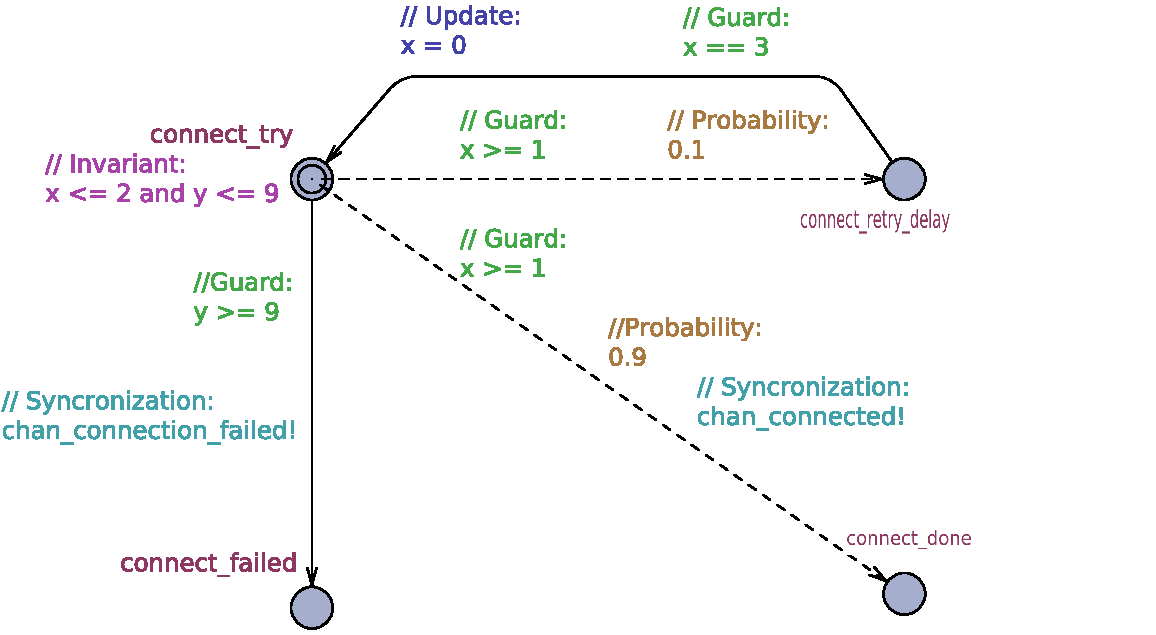
\includegraphics[scale=0.51]{PLP-Verify-ICAPS-2021/examplePta-eps-converted-to-update.pdf}
%%removedVspace
\caption{Example PTA for connection protocol}
\label{fig:examplePTA}
%removedVspace
\end{figure}

\subsection{PTAs}
\par Probabilistic timed automata (PTAs)~\citep{PTA}  model systems with probabilistic and real-time characteristics. They can be viewed
as a combining Markov Decision Processes (MDPs) with a timed-automata.
A PTA contains: 1. Integer-valued variables. 2. Clocks -- non-negative real-valued variables, which all increase at the same rate. 3. Constraints -- boolean combinations of
(in)equalities consisting of sums of clock variables and constants.  4. Locations (the PTA's \textit{nodes}) -- a finite set of locations, with
a distinguished initial location. 5. Actions (the PTA's \textit{edges}) -- a finite set of transitions between locations. 6. Invariant conditions -- constraints on locations. 7. Enabling conditions -- constraints on actions. 8. Probabilities -- transition probabilities of enabled actions. The automaton state consists of the current node and the values of its clocks and variables.

The transition function allows two types of transitions between states: 1. Time transition -- all clocks advance by a certain time interval, while the invariant of the current node is preserved. 2. Action transition -- transition on an enabled edge chosen according to the probability. As part of the transition, the values of variables and clocks can be updated, too. The automaton starts at the initial node and advances along edges according to invariants and enabling conditions. The state of the PTA describes the current location and the clock values. And a run is legal if each next state is reached by a legal transition: either a change in clock value that is permitted by the invariants, or an action transition in which an edge between locations
whose guards are satisfied is traversed and clocks are possibly updated in line with the constraints. The edge probability can be used to associate the likelihood of the transition/run given the action/s.



We use a stronger  PTA variant
supported by UPPAAL. 1. We support urgent nodes -- nodes without time transition such that clocks cannot advance while in them. 2. In basic PTAs, one can only reset clock values to 0. We allow variable values to be updated to any function of other variable values, as well as to a value obtained by sampling some distribution. 3. We use multiple concurrent PTAs. This serves as syntactic sugar,
as they can be encoded as a single product PTA. 4. We allow channels. Channels are used to synchronize the transitions of different PTAs. A channel is tied to an edge and can be used either to send or receive a signal. The action of passing a signal on a channel is immediate. Transition on an edge with the sending end of the channel does not delay the transition on that edge, but transition on an edge with a receiving end of a channel may delay the transition until the signal on the channel is received. In addition, we use real-valued variables for convenience, but model them with finite precision as fractions.


Figure~1 describes in graphical form a PTA for a connection protocol with up to three retries.
There are two clocks: $x$ and $y$. Node \textit{``connect\_try"} is the initial node, with invariant: $x\leq 2\wedge y \leq 9$. At anytime in the interval $\big[0,1\big)$, it is impossible to transition along edges because of the guards (enabling conditions). Up until two time units, the PTA can stay at \textit{``connect\_try"}, but then it must transition on an edge to \textit{``connect\_done"} (with probability 0.9) or \textit{``connect\_retry\_delay"} (with probability 0.1). If it transitioned to \textit{``connect\_done"}, it sends a signal on \textit{``chan\_connect"} channel and remains at \textit{``connect\_done"} state. If it transitioned to \textit{``connect\_retry\_delay"}, it waits for $x$ to become 3, then updates $x$ to 0, and transition to \textit{``connect\_try"} for another connection attempt. If all three attempts to connect fail, the automaton will transition from  \textit{``connect\_try"} to \textit{``connect\_failed"}, send a signal on \textit{``chan\_connection\_failed"} channel, and will remain in \textit{``connect\_failed"} state.
%In our figures, we use the following color codes:
%\frameImage{examplePta.eps}{1.6in}{3.1in}{Example PTA for connection protocol}

%\colorsTable

%endsection{PTAs}



\section{Related Work}
Our semantics for PLPs is obtained by mapping them to a PTA. This type of semantics is sometimes called translation semantics and semantic anchoring. PTAs were used for this purpose in a number of earlier systems: mapping AADL to UPPAAL~\citep{JLPJ12} and mapping RT-DEVS to UPPAAL~\citep{FN08}. Neither of these systems uses the probabilistic aspects of PTAs, and both are part of systems that strive to provide a complete bottom-up approach to robot software design. Our use of PLPs attempts to address systems that use existing, imported, or locally developed components.
More recent work~\cite{FoughaliIS19} translates the code written using the Genom3 platform~\citep{Genom} to timed automata. Like the above systems, Genom3 is a complete platform for
designing robot software. Unlike the above, and similar to our work, this work also introduces the option of using
a probabilistic model of the environment, by essentially learning the frequency of different outcomes within an
originally non-deterministic model. They then use UPPAAL-SMC to do probabilistic
model checking on the resulting PTA. Finally, probably closest to our work is~\cite{Lesire20}.
It describes a language for describing skills that are quite similar to PLPs, although it does not have probabilistic components.
From this description, they can generate PDDL descriptions and use planning to compose skills, much like~\cite{PlanRob16} as well as finite-state machines, which  are then used for verification using the
NuSMV model-checker~\citep{NuSMV}.


The composition of simple components to obtain more complex ones is a basic technique in automata theory, supported by operations such as Cartesian product and automata sequencing~\citep{automatabook}. Tree structures specifically, are often used to describe hierarchical compositions and branching computation. Our work uses these ideas, but supports general graphs with loops.

\begin{figure*}[h]
\centering
%%removedVspace
%\includegraphics[scale=0.43]{ptaAchieve17.eps}
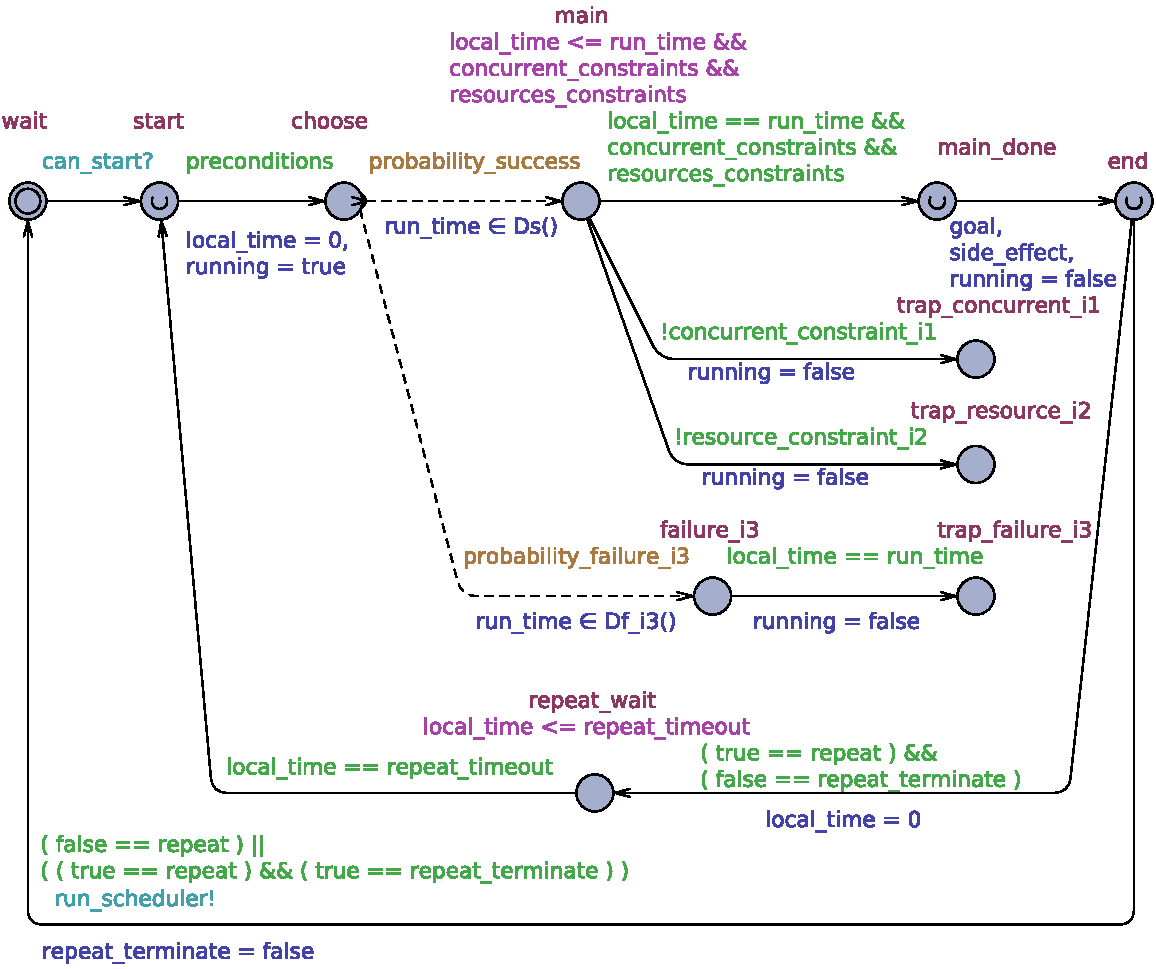
\includegraphics[width=0.58\linewidth]{PLP-Verify-ICAPS-2021/ptaAchieve17-eps-converted-to.pdf}
%%removedVspace
\caption{Template for PTA\textsubscript{PLP} achieve}
\label{fig:ptaAchieve}
%removedVspace
\end{figure*}

The idea of verifying systems viewed as trees or graphs of processes or components is not new in robotics.
In~\citet{SPS00} the authors develop an approach for verifying elements of the Task Description Language (TDL)~\citep{TCA} related to decomposition and synchronisation.
This is done by providing a translation into the SMV model-checking language. In~\citet{AKRB13} behavior networks are verified by using model-checking. In~\citet{vTSL}, TSL, a domain specific language for robotics, which makes use of task trees and hierarchical decomposition, like TDL, is verified by translating its specifications into a Promela model used by the Spin model checker.
More recently, ASPiC~\cite{ASPiC} is a system that allows the composition of simple petri-nets to obtain complex control structures/plans.
Combining the ability to verify petri-nets with the semantics of the composition operators used, the system is able to verify a certain form of soundness.
The basic elements scheduled by these languages differ significantly from PLPs.
First, none of these methods model stochastic elements, while PLPs make use of probabilistic information, and control graphs allow for probabilistic choice, modeling stochastic environments and, consequently, require the use of probabilistic model checking. Second, PLPs offer more information about run-time behavior (e.g., progress measure, run-time distributions), are divided into four categories based on the component's role, yet are not rich enough to actually allow for code generation, as in these methods.



\section{Formal Semantics for PLPs}
Compared to PLPs, PTAs are a much more detailed, program-like description of behavior.
As such, they can be used for code specifications or programming controllers. PLPs, on the other hand,
aim to provide a more abstract, intuitive description of implemented code.
Given this, it is natural to use PTAs as a semantic model for PLPs. Here, we outline a translation
semantics for PLPs by mapping them into PTAs.
Due to space limitations, we provide an overview of the
semantics of Achieve. The complete specification appears in~\citet{kovalchu2018}.\footnote{\normalfont{Available at \emph{https://github.com/a-l-e-x-d-s-9/Thesis2017/blob/master/ThesisToLatex/Thesis.pdf}}}
%While this is a desirable goal for the proper specification of PLPs, it also serves
%as a building block in our approach for the verification
%of complex scripts modeled as control graphs.
%The mapping from PLPs to PTAs is quite technical, so we illustrate its main ideas by describing the PTA schema for an \textit{achieve} PLP. Additional details appear in the Appendix.



%\subsection{Common elements of all PTA\textsubscript{PLP}}
(1) For every PLP type, a distinctive PTA scheme exists, but all
%schemes
share a common structure that we describe here.
\par The successful execution path of each PTA contains the following sequence of nodes: 1. \textit{``wait"} -- waits for the scheduling PTA to let the current PTA command run (i.e., the relevant code modeled by the PLP is starting to execute).%
\footnote{The scheduling PTA captures the controller that selects when to execute a module. Later, we define an explicit scheduler model.
Here, we simply treat it as an external entity that decides when to activate a PLP.}
2. \textit{``start"} -- the scheduling PTA allowed the current PTA command to run. 3. \textit{``choose"} -- the PLP's preconditions hold. 4. \textit{``main"} -- run-time path for a successful execution. 5. \textit{``main\_done"} -- PLP's code terminated. 6. \textit{``end"} -- completed current execution cycle of PTA\textsubscript{PLP}.

\par Node transitions
%between nodes
are as follows: 1. \textit{``wait$\rightarrow$start"} is taken when a signal from the scheduling PTA is received. 2. \textit{``start$\rightarrow$choose"} is taken only if the preconditions are fulfilled. 3.  \textit{``choose$\rightarrow$main"} is taken when the PTA selects (probabilistically) to take the success path. 4. \textit{``main$\rightarrow$main\_done"} is taken when run time is up, and the concurrent and resource related constraints are fulfilled. 5. \textit{``main\_done$\rightarrow$end"} updates  side effects and goal conditions.
However, if the probabilistic choice in the \textit{choose} node leads to a failure path,
%\par Besides its successful execution path,
a PTA\textsubscript{PLP} may end up in one of the PLP’s failure states.
%This occurs if the probabilistic choice in the \textit{choose} node leads to one of the failure path.

(2) For a given set of PLPs representing a certain system, we list all variables, parameters, constants, and resources. Then, we match a PTA\textsubscript{PLP} variable for each and initialized them based on
%according to
the initial values specified in the PLPs. We also create one status variable for each PLP. It is used to
indicate whether the PTA\textsubscript{PLP} is currently running or not.

(3) %Using the PTA\textsubscript{PLP} variables, we can build the conditions used by PLPs.
In PLPs the concept of a \textit{condition} is used in two distinctive ways: 1.  A logical expression  such as $a=b$ that must be satisfied by the external world; for example, a precondition.
2. A logical expression that is made true by the code module modeled by the PLP -- which is essentially an assignment, such as in the case of goal conditions.
\par Logical conditions are transformed to negation normal form, and
are then translated to a PTA guard condition of an appropriate edge in the PTA\textsubscript{PLP}.
Assignments are translated to a PTA update of an edge in
the representative PTA\textsubscript{PLP} according to its role and place in the PLP.%
\footnote{Recall that action transitions perform such updates.}
%\footnote{Note that, in general, one could have goal conditions that are not assignments in a PLP, such as $a<b$.}
%We note that PLP conditions supports existential and universal quantification.
Unfortunately, our translation does not support existential and universal quantifications,
at present.


%\subsection{Modelling Achieve PLP}
%\par We now describe the PTA schema for the {\em achieve} PLP. Many of the ideas here apply to the other PLPs, as is. Some more details about standard mappings and the schema for the other PLP types appear in the appendix.


%\frameImage{ptaAchieve17.eps}{2.76in}{3.32in}{Template for PTA\textsubscript{PLP} achieve}
%\aNote{Clarification about scheduling PTA and channel:}



For a given \textit{achieve} PLP, we create PTA\textsubscript{PLP} achieve, described in Figure~\ref{fig:ptaAchieve}.
PTA\textsubscript{PLP} starts at the initial node, \textit{wait} and
waits for a start signal from the scheduling PTA. When a signal arrives on channel \textit{``can\_start"},
%Scheduling PTA responsible to signal PTA\textsubscript{PLP} to start working with a designated channel.
%\rNote{It is still not clear what the scheduling PTA is. How does it work, why/when does it send a start channel? Is it implementing some control structure?}
%\aNote{In our case, control graph is the scheduling mechanism that schedules PLPs. But in general, "scheduling PTA" can represent Hardware + Firmware + Operating System +   Software that allows execution of the particular module, within the modeling framework. I use here a vague term "scheduling PTA" because control graph will be presented later.}
it transitions to \textit{``start"}.
% occurs when a signal arrives on channel \textit{"can\_start"} from the scheduling PTA.
%\rNote{This is unclear. What is the relation between the channel and scheduling PTA? What does "symbolizes PLP scheduling" mean}
%\aNote{Change above: "Scheduling PTA responsible to signal PTA\textsubscript{PLP} to start working with a designated channel."}
First, we check the PLP's preconditions by a transition  to \textit{``choose"} with guard condition \textit{``precondition"}. Then,
the PTA samples a successful execution or one of the possible failure modes based on the associated probabilities.
If a failure path is chosen, it waits for \textit{``run\_time"} time according to run-time distribution \textit{``Df\_i3()"} in \textit{``failure\_i3"} node and then stays in \textit{``trap\_failure\_i3"} state. If a successful  execution is chosen, it transitions from \textit{``choose"} node to \textit{``main"}.  Time can pass in the \textit{``main"} node according to the run time distribution \textit{``Ds()"} stored in the \textit{``run\_time"} variable.




Even if the current path represents a successful internal execution, external constraints may still force the PLP to fail. This is captured by \textit{``main"}'s invariant condition \textit{``concurrent\_constraints $\&\&$ resources\_constraints"}. In case of failure caused by a concurrent condition, concurrent module, or resource, the PTA transitions to \textit{``trap\_concurrent\_i1"} or \textit{``trap\_resource\_i2"} respectively. If the external constraints are fulfilled while in \textit{``main"}, the transition to \textit{``main\_done"} is possible. Finally, the transition to \textit{``end"} node updates the goal conditions and side effects.
% If a \textit{repeat} mode is enabled, the PTA will transition to \textit{``repeat\_wait"}, and then to \textit{"start"} for another cycle of PTA\textsubscript{PLP} run. If the \textit{repeat} mode is disabled, the PTA will transition to \textit{"wait"}, and will let the scheduler PTA know that it is done by a signal on the \textit{"run\_scheduler"} channel.


\par PLP logical conditions are converted to PTA guard conditions
as follows: 1. Preconditions to \textit{``preconditions"}. 2. Concurrency conditions and concurrent modules constraints are transformed into $m\textsubscript{1}$ statements that are conjoined to form \textit{``concurrent\_constraints"}. For each statement $i\textsubscript{1} \in \big[ 1, m\textsubscript{1} \big]$ there is a path to \textit{``trap\_concurrent\_i1"} from \textit{``main"} with a guard \textit{``!concurrent\_constraint\_i1"}.
%\aNote{1. Yes, there are m1 paths leading to m1 traps (similarly for m2 and m3), that’s why I use locations with indexes. I’m not sure why but the explanation about m3 is commented out right before Maintain subsection. 2. Yes, the "AND" on all constraints make them one big constraint. I use another variable and not the constraints just to minimize the text in the PTA schema. 3. I use the m1/2/3 only here to specify that it’s not a single case, and differentiate between them.}
%
3. Required resources are gathered into $m\textsubscript{2}$ statements and conjoined to form the \textit{``resources\_constraints"}. For each statement $i\textsubscript{2} \in \big[ 1, m\textsubscript{2} \big]$, there is a path to \textit{``trap\_resource\_i2"} from \textit{``main"} with a guard \textit{``!resource\_constraint\_i2"}. 4. The \textit{Repeat} state of a PLP is represented by a boolean variable \textit{``repeat"}.
\par Assignment conditions in the PLP are converted to assignments in the PTA as follows: 1.
The transition between \textit{``main\_done"} to \textit{``end"} updates the
PLP's goal condition to true. (This is the ``goal" statement there.)
2. The definition of side effects in PLPs does not specify the time in which the side effect occurs,
and we therefore decided to make this change immediately before the PTA
completes the transition between  \textit{``main\_done"} and \textit{``end"}.
\par Constraints between concurrent modules are enforced by using
the \textit{``running"} status variable. This is a flag that indicates, for each PTA\textsubscript{PLP}, whether its underlying module is currently being executed.
%It is \textit{true} while the PTA emulates the PLP’s running state,
Every PTA can include guard conditions that refer
to the running state of another PTA, and thus either restrict or
require its concurrent execution.
%\par We assume there are $m\textsubscript{3}$ failure states for PLP, each one represented by $i\textsubscript{3} \in \big[ 1, m\textsubscript{3} \big]$ path leading to \textit{"failure\_i3"} with probability \textit{"probability\_failure\_i3"}.


\commentout{
\subsection{Maintain}

\begin{figure}[]
\centering
%%removedVspace
\includegraphics[scale=0.43]{ptaMaintain17.eps}
%%removedVspace
\caption{Template for PTA\textsubscript{PLP} maintain}
\label{fig:ptaMaintain}
%removedVspace
\end{figure}

%\frameImage{ptaMaintain17.eps}{2.16in}{3.32in}{Template for PTA\textsubscript{PLP} maintain}
PTA\textsubscript{PLP} \textit{maintain}, shown above in  Figure~\ref{fig:ptaMaintain}. is similar to PTA\textsubscript{PLP} \textit{achieve} with a few changes:
%1. No repeat path -- because PLP maintain does not support \textit{repeat}.
1. An additional node \textit{``wait\_maintain\_true"} that models the time needed by PLP Maintain for the maintained condition to become true.
2. The condition maintained by the PLP is converted to an assignment (to model the change caused by the underlying module). This assignment appears here as \textit{``maintained"}, which is an update on a transition from \textit{``wait\_maintain\_true"} to \textit{``main"} node.
3. Successful termination of the PLP is accomplished by the \textit{``termination\_success"} condition that can force a transition to \textit{``main\_done"}. 4.  Unsuccessful termination is accomplished by the \textit{``termination\_failure"} condition that can force a transition to \textit{``trap\_failure\_termination"}.
\par In the template above, the PTA\textsubscript{PLP} maintain implements the maintained condition (i.e., forces it to be \textit{true})
using the \textit{``maintained"} assignment.
This is done only once, before \textit{``main"} node. It is also possible to
%enforce an additional behaviors: 1. Make
ensure that the assignments in \textit{``maintained"} are not overwritten with other values during the execution of the PTA. This can be accomplished by converting the \textit{``maintained"} assignments to a logical condition in the invariant of the \textit{``main"} node, and creating a failure state in case it changes while in \textit{``main"}.
%2. We can enforce the \textit{``maintained"} assignment by converting the \textit{"main"} node into two nodes and forcing a transition every some fixed interval of time. Each such transition will write the \textit{"maintained"} assignment.
%\rNote{The first option seems clean. The second seems more like a hack?}
%\aNote{Yes, we discussed it some time ago.}

\commentout{
\subsection{Observe}
\frameImage{ptaObserve17.eps}{2.76in}{3.32in}{Template for PTA\textsubscript{PLP} observe}
\par PTA\textsubscript{PLP} \textit{observe}, shown above, is similar to PTA\textsubscript{PLP} \textit{achieve} except for a change in the transition between \textit{``main\_done"} and \textit{``end"}, which now assigns one
of the possible values to the observed variable.
By default, the choice is uniform, although alternative distributions can be supported.
%\rNote{Is this a non-deterministic choice? Probabilistic?}
%\aNote{Non-deterministic choice / Equal probabilities.}
%\rNote{Non-deterministic and equal probabilities is not the same. Which is it?}
%\aNote{In the model that we use when probabilities of edges not specified, it means that all outgoing edges have an equal probability. In UPPAAL - "Uppaal SMC Tutorial": http://people.cs.aau.dk/~kgl/SSFT2015/SMC\%20tutorial.pdf "The modeling formalism of Uppaal SMC is based on a stochastic interpretation and extension of the timed automata (TA) formalism [AD94] used in the classical model-checking version of Uppaal [?]. For individual TA components the stochastic interpretation refines the non-deterministic choices between multiple enable transition by probabilistic choices (that may or may not be user-defined). Similarly, the non-deterministic choices of time-delays are refined by probability distributions, which at the component level are given either by uniform distributions in cases of time-bounded delays or by exponential distributions (with user-defined rates) in cases of unbounded delays."}
}

\subsection{Detect}
\frameImage{ptaDetect17.eps}{2.3in}{3.32in}{Template for PTA\textsubscript{PLP} detect}
\par PTA\textsubscript{PLP} \textit{detect}, shown above, is similar to the previous PTAs\textsubscript{PLP} with the following changes: 1. There is only one internal failure path. 2. There is no time distribution for the success path; only termination with a positive outcome.

\subsection{Failure handling}
\par Currently, all failures lead to a trap state. This design choice essentially says that any failure is fatal. It is motivated by the
need to focus on path with zero internal PLPs failures. To address systems with a failure recovery mechanism, we can change the PTA\textsubscript{PLP} design so that trap states may still lead to a completion of the PTA\textsubscript{PLP}, but without achieving the goals and the side effects.
}
%endsection{A Formal Semantics for PLPs}

%\begin{figure}[htb!]
%\centering
%%removedVspace
%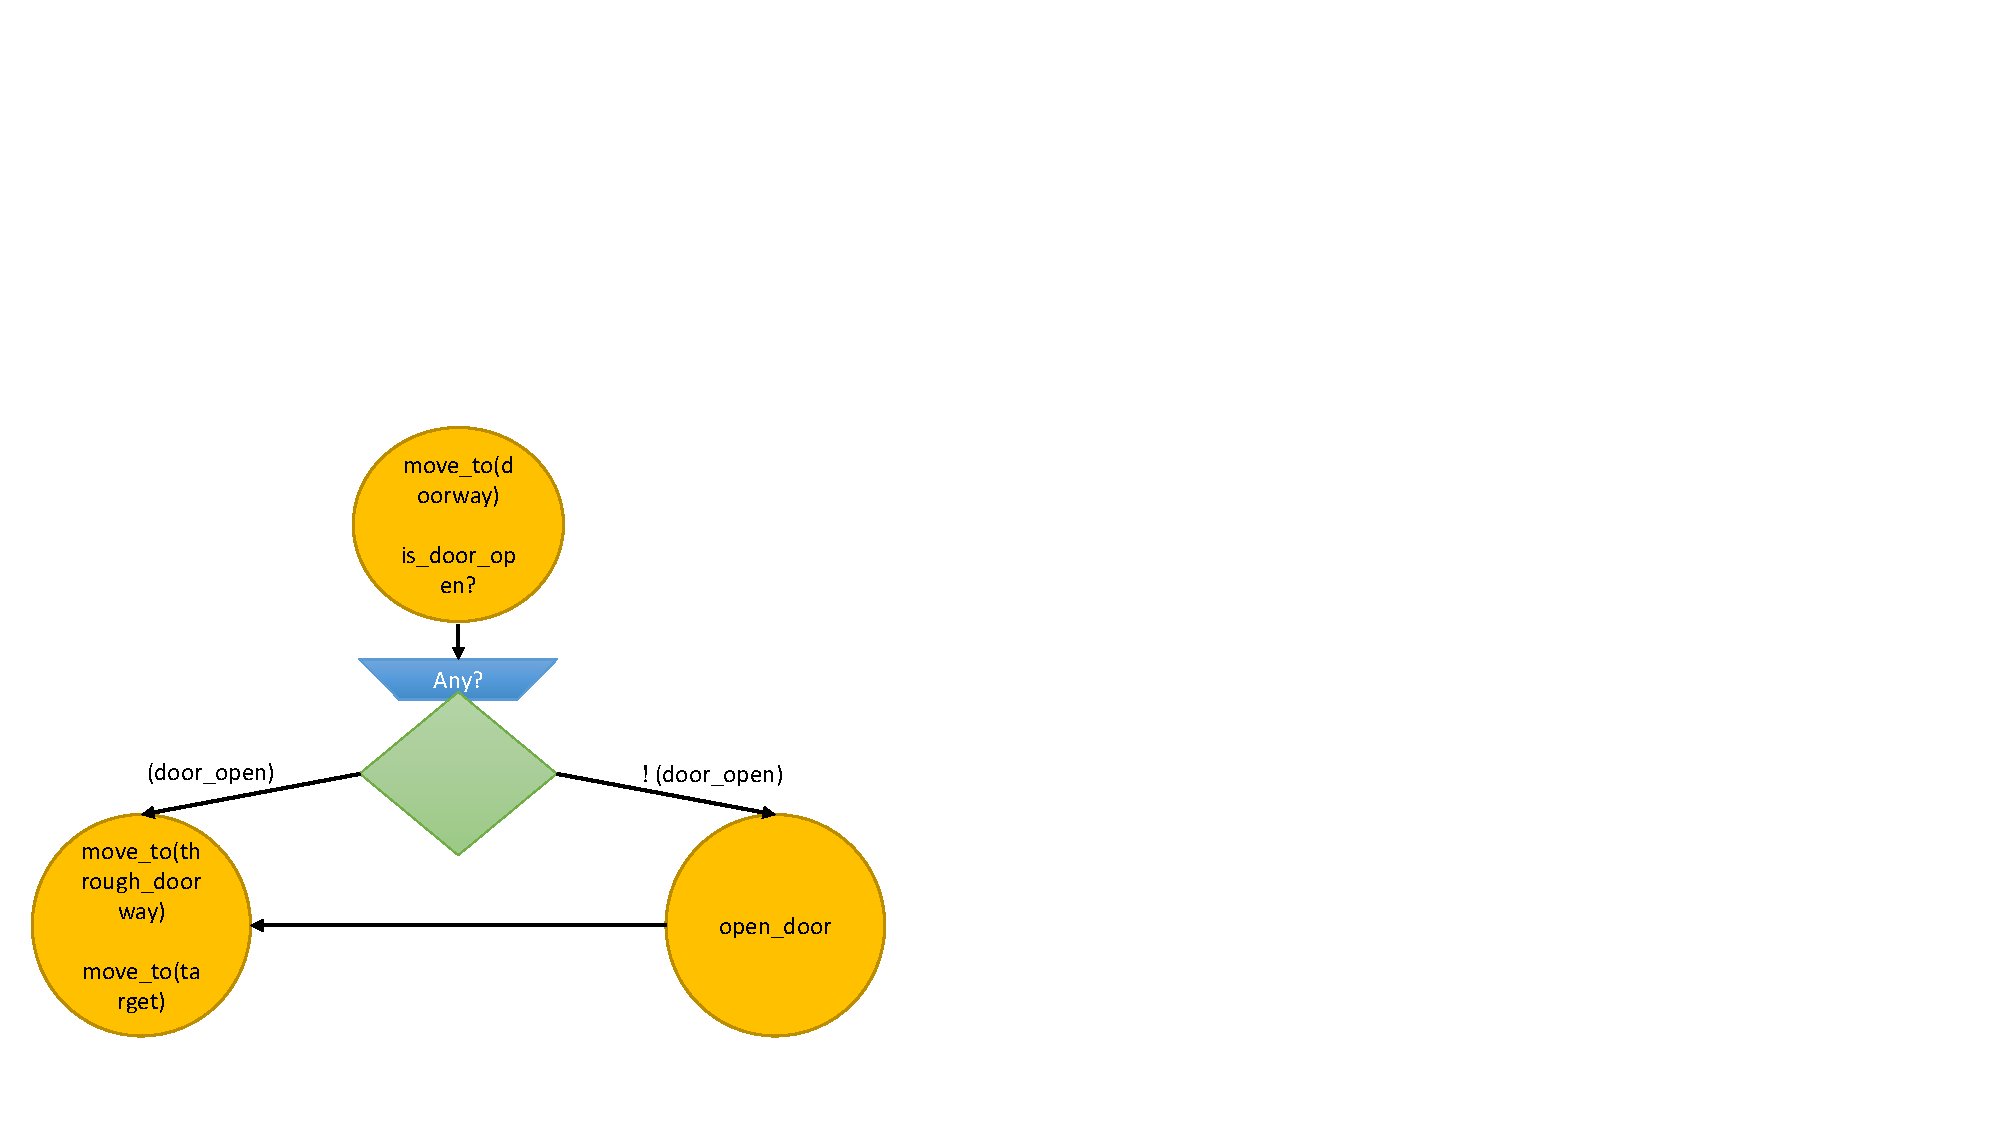
\includegraphics[width=0.73\linewidth]{PLP-Verify-ICAPS-2021/example1ControlGraph-1.pdf}
%%removedVspace
%%removedVspace
%\caption{Example of a control graph}
%\label{fig:example1}
%%removedVspace
%\end{figure}

\section{Verifying Complex Controllers}
%The mapping from PLPs to PTAs allows us to leverage existing verification tools to verify controllers.
%The idea is as follows:
Given a controller that calls different code modules, for each of which we have a PLP, we generate a set of interacting PTAs that represent the entire program. These PTAs can be fed into UPPAAL-SMC~\cite{UPPAAL-SMC}, a PTA verification tool, which can be queried to verify various conditions. Below we describe our formalization of such controllers and the main ideas behind their mapping to PTAs.
%See~\cite{kovalchu2018} for additional details.
\subsection{Control Graphs}
\label{S:control}
We use {\em control graphs} to describe   algorithms controlling execution of robotic modules specified by PLPs.
%They allow for probabilistic and conditional branching, as well as parallel execution.
%
A control graph is a directed graph with a single root node in which execution starts. Each node
represents a call to some code modules. Transitions between nodes depend on the system state obtained when the parent node(s) terminates execution. They can be stochastic or conditional on the current state.

There are four types of control nodes: 1. PTA\textsubscript{PLP} launcher nodes launch a sequence of PTA\textsubscript{PLP} that executes one at a time. 2. Probabilistic nodes choose a single edge to proceed with based on the edge's probability. This allows implementing methods that require some randomization, e.g., to escape from cycles.
3. Conditional nodes choose a single edge to proceed with. Only an edge whose condition is satisfied can be selected. If more than one edge condition is satisfied, one is selected non-deterministically.
(If no condition is satisfied, then this is viewed as a failure.)
%\rNote{What happens if no condition is satisfied?}
%\aNote{If PTA must transition but can’t, it will be regarded as deadlock by UPPAAL, UPPAAL will try other paths.}
4. Concurrent nodes execute all nodes reached by their outdoing edges concurrently.
Finally, each node type comes in two variations: 1. Starts only when \textbf{all} of its immediate parents terminated. 2. Starts whenever \textbf{at least one} of its parents terminated. Nodes in the control graph can update the value of variables that are used both by PTA\textsubscript{PLP} and other nodes in the control graph.

An important aspect of control graphs is the ability to express loops by allowing backward edges. This allows us to specify a much larger class of algorithms. Circular execution can be ended by a probability node or a conditional node.

%To support loop extension simple changes to the previous description are made that allow running the same control node multiple times by appropriately resetting flags.



%Figure~\ref{fig:example1} illustrates a control graph for an autonomous robot that needs to
%with an arm whose task is to move the robot
%move from one room to another through a doorway. The door is not locked and can be either open or closed. The control graph refers to three PTAs\textsubscript{PLP}: 1. move\_to({doorway $\vert$ target $\vert$ through\_doorway}) -- moves the robot according to its parameter. 2. is\_door\_open -- checks if the door is open. 3. open\_door -- opens the door.
%\frameImage{example1ControlGraph.png}{3.2in}{2.4in}{Example of a control graph}
%This control graph starts with a node that executes move-to-doorway and checks if the door is open. Then, it uses a conditional node to check if the door should be opened. In case the door is closed, it opens the door. Eventually, it moves through the doorway to the target at the other room.

%\rNote{Please replace "*" with "Op" or "OP"}
%\aNote{Done.}
%\aNote{Is it better now?}


%\rNote{By circular execution you mean an edge backwards? Is the possibility of running the same control node multiple times something important? difficult?}
%\aNote{Yes, you can call it an edge backward. The capacity to run the same node more than once is the core part that allows circular execution. In the paper, presented nodes can run only once, so I mention the change needed for this extension to work. This is not a difficult change. Basically, I reset flags from predecessors, and at the last state I add an edge to the first state, also I handle edge case of all flags enabled before the node is done so it would not wait for signals.}

%, it can be achieved by the following changes in PTAs\textsubscript{Node} definitions: 1. We remove the usage of channels between PTAs\textsubscript{Node} to signal when to start. 2. In the node \textit{"init\_node"} we add invariant: for AND nodes -- invariant is a logical disjunction on predecessors’ pass statuses; for OR nodes -- invariant is a logical conjunction on predecessors’ negation of a pass statuses. 3. The transition from \textit{"init\_node"} to  \textit{"wait"},
%endsection{Control Graphs}

%\begin{figure}[hbt!]
%\centering
%%%removedVspace
%\includegraphics[scale=0.33]{controlTree1.eps}
%%%removedVspace
%\caption{First Part of First Control Graph}
%\label{fig:controlTree1}
%%removedVspace
%\end{figure}

\begin{figure}[]
\centering
%%removedVspace
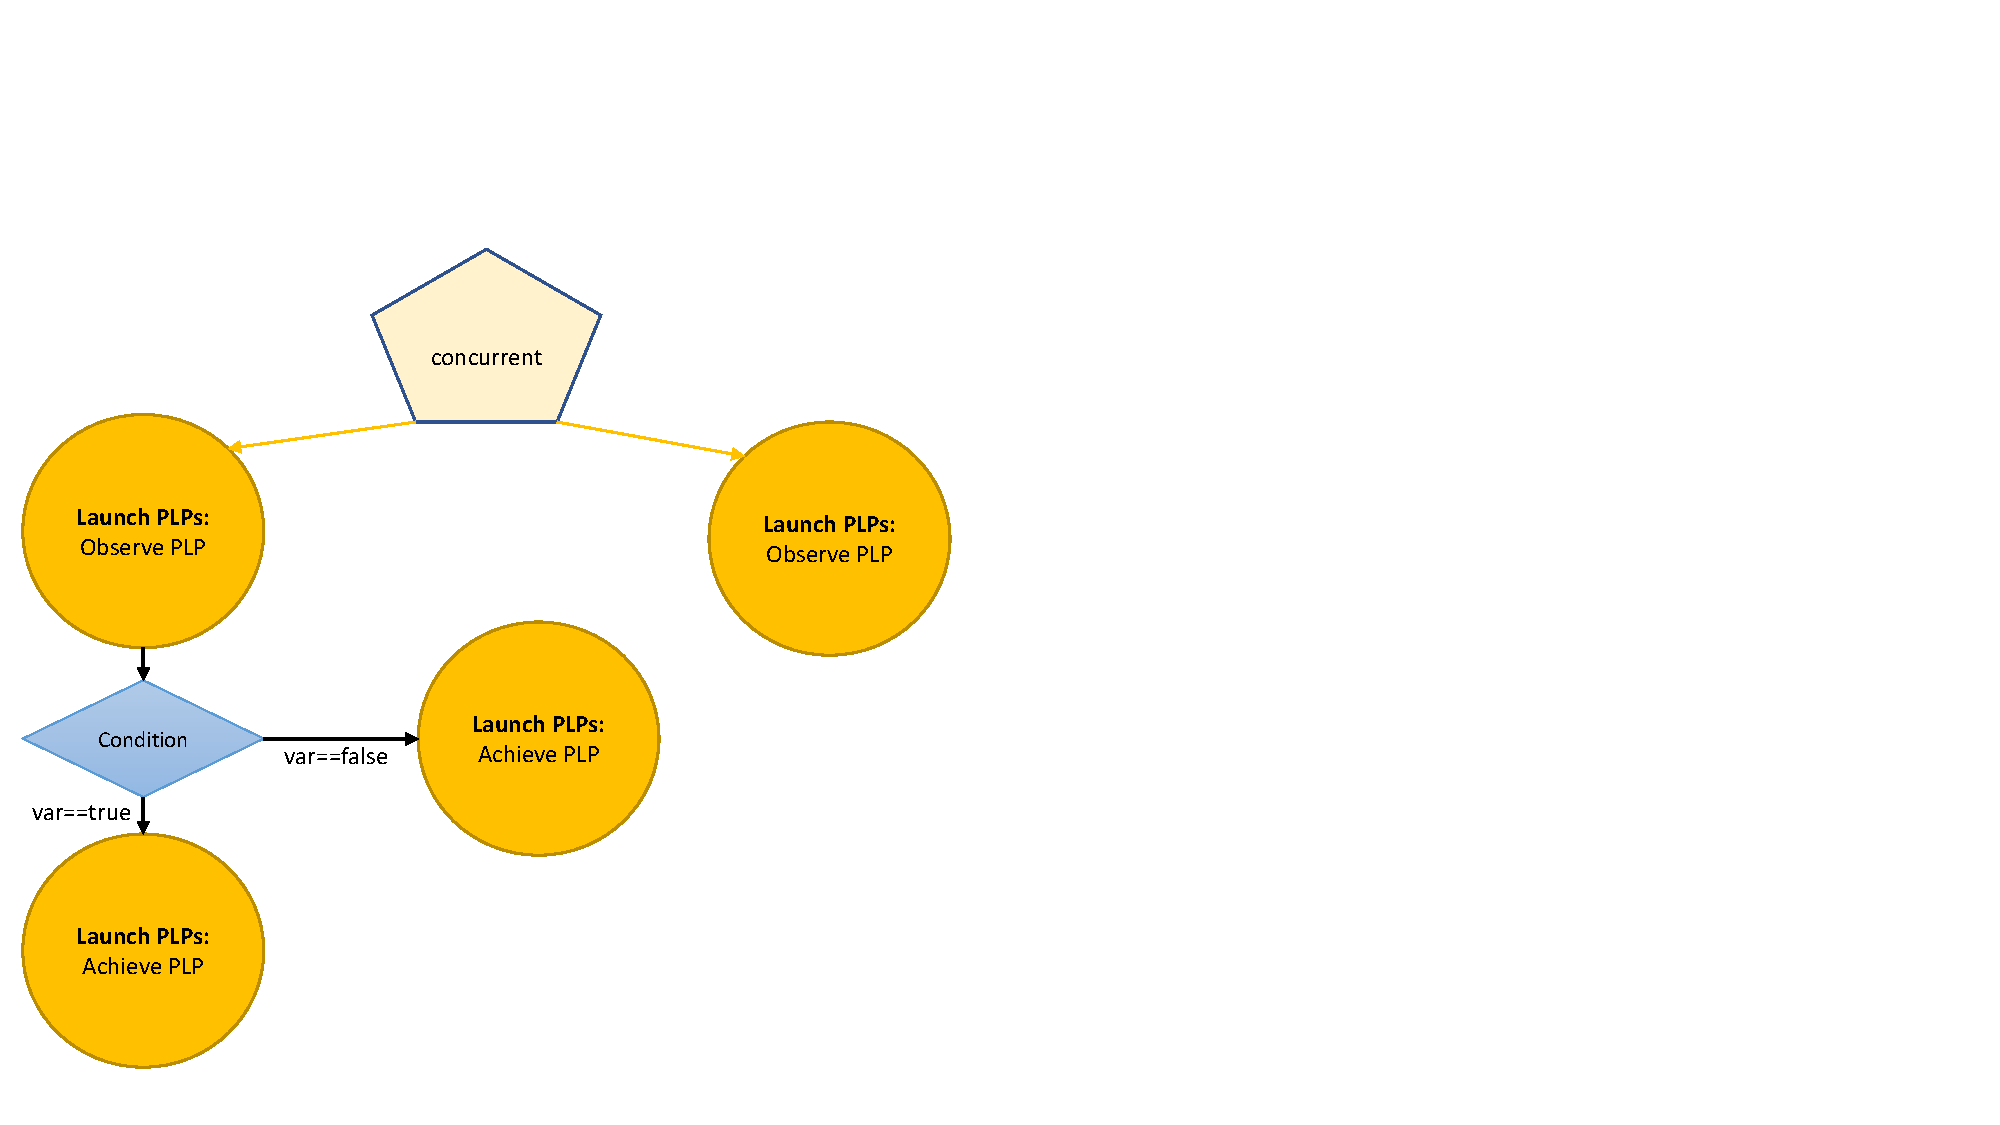
\includegraphics[scale=0.5]{PLP-Verify-ICAPS-2021/controlTree2.pdf}
%removedVspace
\caption{Second Part of First Control Graph}
\label{fig:controlTree2}
\end{figure}

\begin{figure*}[h]
\centering
  \includegraphics[width=0.635\linewidth]{chartQueryExistDuration.pdf}
  %removedVspace
  \caption{Average Time for $\exists$ Query}
  \label{fig:time-exists}
\end{figure*}


\subsection{The Control Graph Verifier}
To verify control graphs with PLPs, we produce a set of PTAs representing this system. We then use UPPAAL-SMC  to answer queries about the system. UPPAAL is a software package for modeling, validation, and verification of real-time systems modeled as networks of timed automata, extended with data types~\citep{BehrmannDLHPYH06}. UPPAAL-SMC is its extension for stochastic model checking.


UPPAAL allows us to query temporal properties of the whole system such as: 1. Possible reachability: Is there an execution path in which $p$ will be eventually true? 2. Guaranteed reachability: Will $p$ be eventually true in all execution path? 3. Safety: Will $p$ be true at all times in all execution path? 4. Possible safety: Is there an execution path in which $p$ will always hold? 5.  Conditional versions of 1-4.
%(E.g., is it the case that for all path, once $p$ holds, $q$ will be eventually true?)
6. Probability of reachability: What is the probability that $p$ will eventually be true? 7. Probability of an invariant: What is the probability that $p$ will always be true?

Queries of the form 6 and 7 are the most interesting from the robotics perspective. Queries of type 6 allow us to ask what is the probability that we will reach a certain goal state with the given controller. For example, what is the probability that coffee will be served eventually? They also allow us to quantify the probability of a particular risk.
For example, what is the probability that we will run out of gas? Queries of type 7 allow us to ask safety queries: what is the probability that some invariant will be maintained throughout execution, e.g., what is the probability that our autonomous car will not take part in an automobile accident?

To convert control graphs to a network of PTAs, we associate a PTA with each node of the graph (PTA\textsubscript{Node}). PTAs\textsubscript{Node} exist alongside PTAs\textsubscript{PLP} and can influence each other through shared variables and channels.
This (quite technical) mapping appears in~\cite{kovalchu2018}.


%endsection{Implementation - Control Graph Verifier}



\section{Empirical Evaluation}
To evaluate our implemented system's performance and scalability,
we run a scalability study and a use-case study.
%Our evaluation includes a study of scalability and a use-case.
%\shashank{~Will we keep this reference?}




%\frameImage{controlTree1.eps}{1.7in}{3in}{First part of the control graph consisting of a binary tree of probabilistic nodes}
%


%
%\frameImage{controlTree2.eps}{2.52in}{2.25in}{Second part of the control graph with the PLPs’ logic}



%\begin{figure}[t]
%\centering
%%%removedVspace
%
\includegraphics[scale=0.38]{controlScalable.eps}
%%%removedVspace
%\caption{Control graph with $j$ PLPs}
%\label{fig:controlScalable}
%%removedVspace
%\end{figure}

\commentout{
\begin{figure*}[ht]
\centering
\begin{subfigure}{.46 \textwidth}
  \centering
  % include first image
  \includegraphics[width=.93\linewidth]{chartCompilationDuration}
  \caption{Average Compilation Time}
  \label{fig:compilation}
\end{subfigure}
\begin{subfigure}{.46 \textwidth}
  \centering
  % include second image
  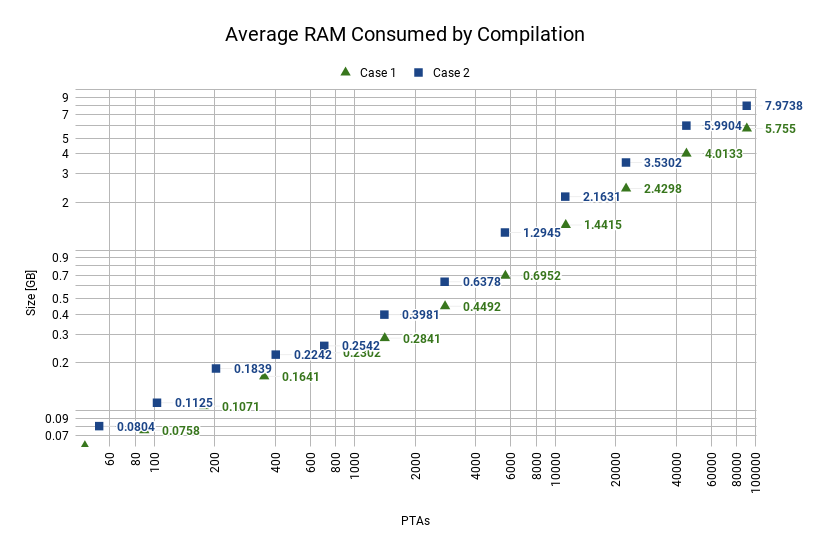
\includegraphics[width=.93\linewidth]{chartCompilationRAM}
  \caption{Avg. RAM Consumed by Compilation}
  \label{fig:RAM}
\end{subfigure}
\caption{Compilation Time and Memory}
\label{fig:compilation-time-memory}
\end{figure*}
}

%%above are the commented out original graphs
\begin{figure*}[h]
\centering
%\begin{subfigure}{.46 \textwidth}
  %\centering
  % include first image
 \includegraphics[width=.63\linewidth]{PLP-Verify-ICAPS-2021/chartCompilationDuration.pdf}
 %removedVspace
\caption{Average Compilation Time}
  %\label{fig:compilation}
%\end{subfigure}
% \begin{subfigure}{.46 \textwidth}
%   \centering
%   % include second image
%   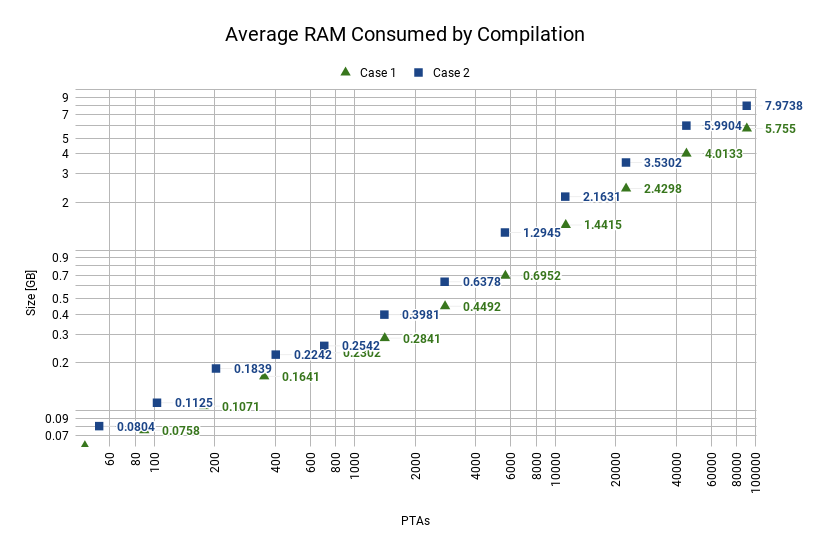
\includegraphics[width=.93\linewidth]{chartCompilationRAM}
%   \caption{Avg. RAM Consumed by Compilation}
%   \label{fig:RAM}
% \end{subfigure}
% \caption{Compilation Time and Memory}
\label{fig:compilation-time}
\end{figure*}

\begin{figure*}[htb!]
  \centering
  % include third image
  \includegraphics[width=0.64\linewidth]{chartQueryProbabilisticDuration.pdf}
  %removedVspace
  \caption{Average Time for Probability Query}
  \label{fig:time-prob-query}
\end{figure*}
% \begin{figure}
%   \centering
%   % include fourth image
%   \includegraphics[scale=0.35]{chartQueryProbabilisticRAM.pdf}
%   \caption{Avg. RAM Consumed for Prob. Query}
%   \label{fig:ram-prob-query}
% \end{figure}
%%%%%

% \begin{figure}[]
% \centering
%   \includegraphics[scale=0.3]{chartCompilationDuration}
%   \caption{Average Compilation Time}
%   \label{fig:compilation}
% \end{figure}
% \begin{figure}
%   \centering
%   % include second image
%   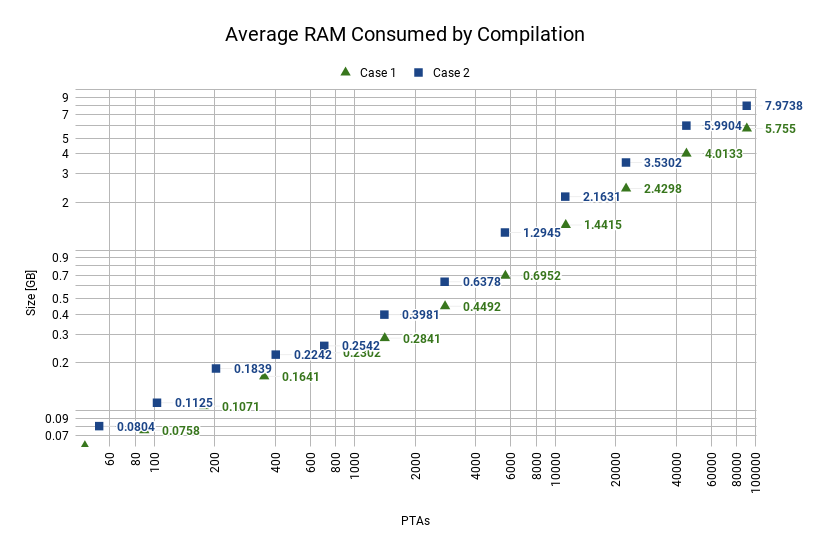
\includegraphics[scale=0.3]{chartCompilationRAM}
%   \caption{Avg. RAM Consumed by Compilation}
%   \label{fig:RAM}
% \end{figure}
%\caption{Compilation Time and Memory}
%\label{fig:compilation-time-memory}
%\end{figure*}

We evaluate resource demands of the system
%by examining both
in two phases: The first phase evaluates
the scalability of the compilation to UPPAAL of the  PTAs associated
with the control graph and its PLPs.
%varying the number of variables,
%We expect compilation time to grow
%with more variables, complex conditions, complex and larger PLPs and control graph.
The second phase evaluates the scalability of
verification queries on the
%an already
compiled system.
%in UPPAAL.
%The query phase is performed on a single file that contains the PTAs that correspond to all the initial PLPs and control nodes.
%in the representative PTAs that recognized by UPPAAL,
%With larger and more complex graphs of PTAs, we expect
%UPPAAL will require more time and more memory to answer queries.

To evaluate
%the practical restrictions of the system in
both phases we use two independent test cases.
The first test case is a comprehensive control graph
with most of our functional elements, all types of control nodes and all PLPs types except {\em detect PLP}. The control graph
%of this system
%is composed of two conceptual parts:
%The first part is
consists of a full binary tree of probabilistic nodes, such that
each of its leaf nodes
is associated with the independent control sub-graph shown in Figure~\ref{fig:controlTree2}.
By controlling the binary tree's height,
we  change the graph's size.


%Our generator takes the desired height of the tree,
%and generates a control graph
%as shown in Figure~\ref{fig:controlTree1},
%whose number leaf sub-graphs is exponential on its height.
The root node of the sub-graph associated with each leaf node
%in this sub-graph
allows concurrent execution of two paths: the first path contains a {\em maintain} PLP that maintains a certain condition needed by the other execution path. The other execution path
executes an {\em observe} PLP, which is followed by a conditional node whose choice depends
on the previously observed variable. This conditional node leads to the execution of an {\em achieve} PLP that achieves a certain goal, but it also requires the concurrent {\em maintain} PLP to run at the same time.

The second test case  is a  simple control graph with a single node that launches a sequence of PLPs. All PLPs are functionally identical but recognized by the system as unique.
%\frameImage{controlScalable.eps}{1in}{1in}{Control graph with $j$ PLPs}
It is an extreme form of a PTAs tree, with all PTAs concentrated along a single path, contrary to the first test case with a full and balanced tree of PTAs. The first test case can be more challenging to compile due to an abundance of elements and connections. The second test can be more challenging for query evaluation.
% \par Each PLP contains \footnote{Source file for this example are available at
%{\tt https://github.com/a-l-e-x-d-s-9/plps_verification/tree/master/Examples/example_scalability_test%}
%} a basic {\em achieve} PLP scheme, with single failure case. Therefore, the produced PTA\textsubscript{PLP} for UPPAAL is relatively simple but it contains all the essential parts of typical {\em achieve} PTA\textsubscript{PLP} scheme. This system allows us to test PLPs to PTAs compilation duration and memory usage with various amounts of PLPs, also we can test memory usage of queries.

The results presented below were obtained on a system running an Intel Core i7-4700MQ CPU, 2.40GHz $\times$ 8 with 16 GB RAM, SSD, Java 1.8.0 171, and Ubuntu 17.10 64bit. We used
%the 64bit version of UPPAAL (specifically
``verifyta" -- terminal based query verifier of UPPAAL for Linux -- 4.1.19. Results are averaged over ten runs.
%\cite{kovalchu2018} contains a few additional details.
% The first table describes the results of the compilations of the control graph and PLPs to the UPPAAL system with different amounts of PLPs:

Generally, every PLP and {\em control node} in the system are converted to a single PTA in UPPAAL. In the first test case, this number increases exponentially with height.  To make the two test cases comparable, in the second test case we use a total number of PTAs similar to the first.
%The proportions between PLPs and {\em control nodes} vary between the two test cases and are shown in Figure~\ref{fig:proportion}.


%\begin{figure}[t]
%\centering
%%%removedVspace
%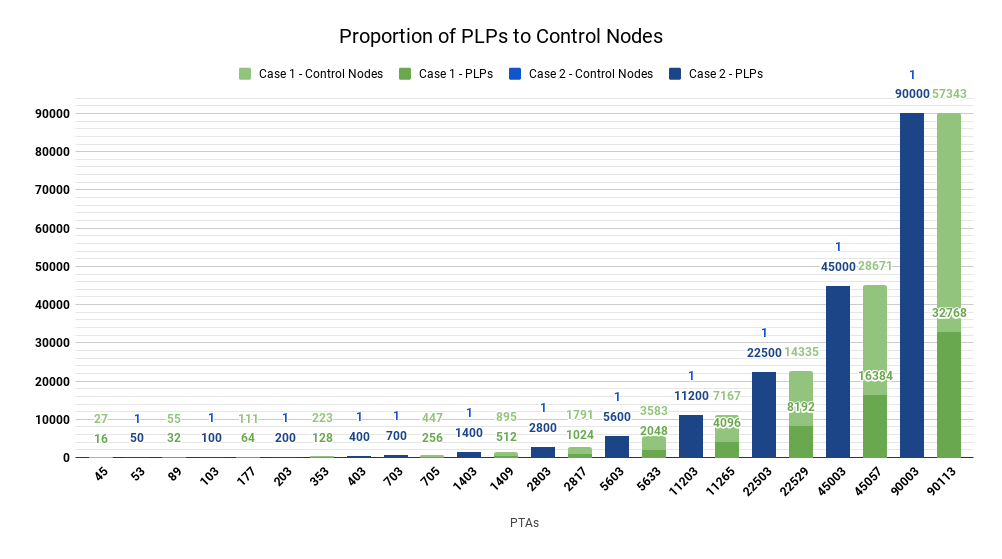
\includegraphics[scale=0.18]{chartPLPsAndControlNodes.png}
%%%removedVspace
%\caption{Proportion of PLPs to Control Nodes}
%\label{fig:proportion}
%%removedVspace
%\end{figure}


%\begin{figure}[t]
%\centering
%%removedVspace
%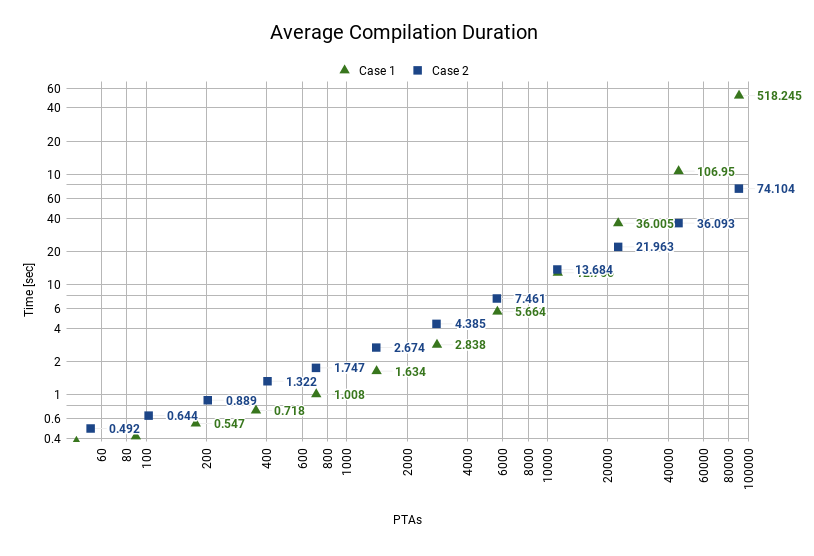
\includegraphics[scale=0.30]{chartCompilationDuration.png}
%%%removedVspace
%\caption{Average Compilation Time}
%\label{fig:compilation}
%%removedVspace
%\end{figure}

%%%%%
% \begin{figure*}[t]
% \centering
%   \includegraphics[width=0.6\linewidth]{chartQueryExistDuration.pdf}
%   %removedVspace
%   \caption{Average Time for $\exists$ Query}
%   \label{fig:time-exists}
% \end{figure*}

% \begin{figure}
%   \centering
%   % include second image
%   \includegraphics[scale=0.35]{chartQueryExistRAM.pdf}
%   \caption{Avg. RAM Consumed for $\exists$ Query}
%   \label{fig:ram-exists}
% \end{figure}
%\caption{Time and memory consumption for $\exists$ UPPAAL queries.}
%\label{fig:uppaal-exists}
%\end{figure*}



We tested the compilation process with up to 90,000 PTAs, although  we cannot envision, in the near future, a system with more than a few dozen components. For 90,000 PTAs, compilation %time was less than 6/8 seconds and required less than 1GB and 0.5GB of RAM  for cases 1 and 2, respectively. For a more realistic, but still
large number of 1000 PTAs
compilation
%time was approximately 0.25 seconds and
required  7.2MB and 4MB of RAM for cases 1 and 2, respectively.
Figure~\ref{fig:compilation-time}
%and~\ref{fig:RAM}
describes the run-time %and memory consumption
of the compilation process.
%s of the {\em control nodes} and PLPs to an UPPAAL system
%for both test cases as a function of the number of PTAs in the system (axes are logarithmic).
%\frameImage{chartCompilationDuration.png}{2.2in}{3.2in}{Average compilation duration}
%\frameImage{chartCompilationRAM.png}{2.2in}{3.2in}{Average RAM consumed by compilation}
%
The results clearly indicate that compilation, a one-time process, is quick and scales to very large problems.
%We cannot envision, in the near future, a system with more than a few dozen components, hence compilation will not be a bottleneck.

%\begin{figure}[t]
%\centering
%%%removedVspace
%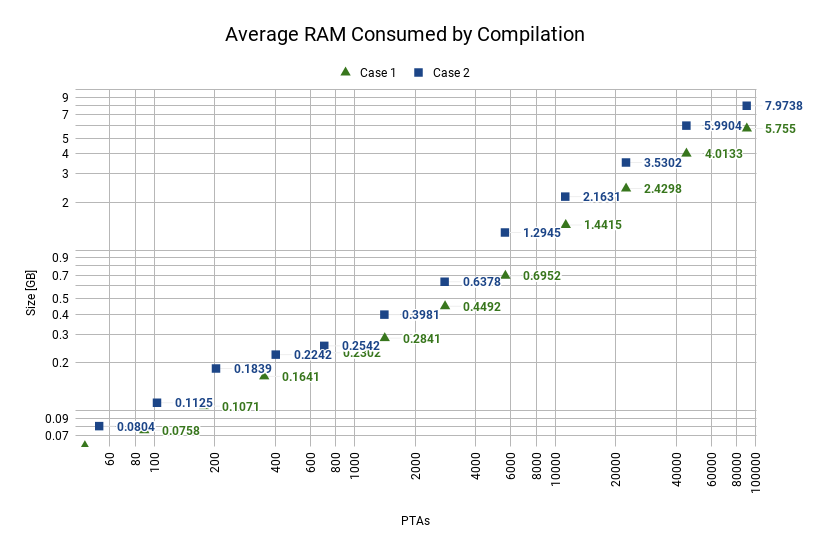
\includegraphics[scale=0.30]{chartCompilationRAM.png}
%%%removedVspace
%\caption{Average RAM Consumed by Compilation}
%\label{fig:RAM}
%%removedVspace
%\end{figure}

%\begin{figure}[t]
%\centering
%%%removedVspace
%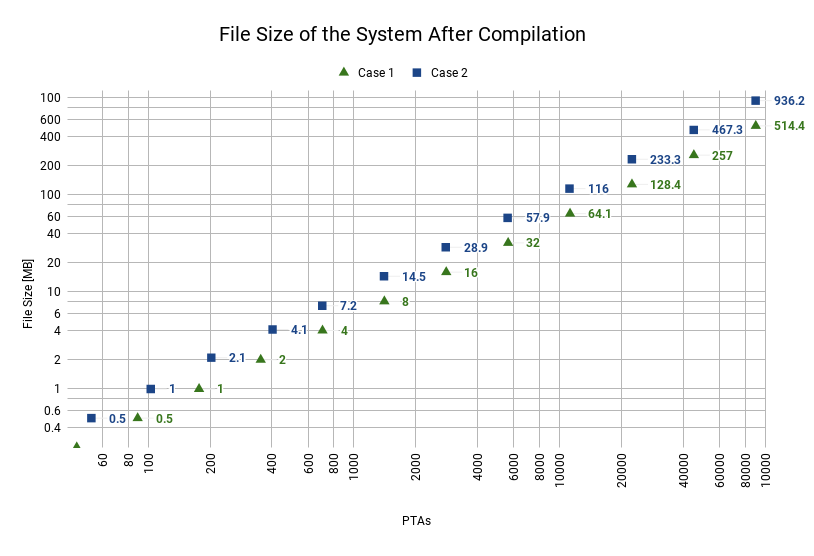
\includegraphics[scale=0.2]{chartUPPAALSystemFileSize.png}
%%%removedVspace
%\caption{File Size Following Compilation}
%\label{fig:size}
%%removedVspace
%\end{figure}
%%\frameImage{chartPLPsAndControlNodes.png}{1.8in}{3.2in}{Proportion of PLPs to Control Nodes}

%The compilation process produces a single file for UPPAAL of manageable size. Even with as many as 90,000 PTAs,
%the file size is smaller than 1GB, and its reduces at
%an exponential rate as we consider (the more realistic) case of fewer PTAs.
%As can be seen in Figure~\ref{fig:size}, even  a system with 90,000 PTAs produces files of size smaller than 1GB.
%\frameImage{chartUPPAALSystemFileSize.png}{2.2in}{3.2in}{System file size following compilation}



Once the system is compiled, we can test its properties using UPPAAL queries. The time and memory needed  by UPPAAL depends on the query and on the properties of the PTAs graph affecting the length of paths and number of paths needed to evaluate the query. Therefore, results for specific query types may vary even in the same system.

% \begin{figure}[t]
% \centering
% %%removedVspace
% \includegraphics[scale=0.30]{chartQueryExistDuration.png}
% %%removedVspace
% \caption{Average Time for $\exists$ Query}
% \label{fig:exists-time}
% %removedVspace
% \end{figure}


% \begin{figure}[t]
% \centering
% %%removedVspace
% \includegraphics[scale=0.3]{chartQueryExistRAM.png}
% %%removedVspace
% \caption{Avg. RAM Consumed for $\exists$  Query}
% \label{fig:exists-memory}
% %removedVspace
% \end{figure}


%\frameImage{chartQueryExistDuration.png}{1.8in}{2.6in}{Average existence query duration.}
%\frameImage{chartQueryExistRAM.png}{1.8in}{2.6in}{Average RAM consumed by existence query}

First, we evaluate a path existence query (``$E<>$").
%\rNote{Do not understand next sentence}
%\aNote{It's a query to test that there is a path from root vertex to a leaf of the execution tree, the root is an initial node in the control graph, and the leaf is the PTA\textsubscript{PLP} on the longest path from the root.}
For both test cases, we test whether the system can reach the most distant PTA\textsubscript{PLP} from the initial state.
%
Run time is
%by the query
%are
shown in Figure~\ref{fig:time-exists}. %and~\ref{fig:ram-exists}.
%~\ref{fig:exists-time} and~\ref{fig:exists-memory}.
Query cost does not scale up as well as compilation cost,
and systems with over 700 PTAs cause UPPAAL to crash due to stack overflow. Yet,  for moderate system sizes, it is relatively efficient, and multiple queries can be carried out in reasonable time. In fact, in systems with $\leq  200$ PTAs, online queries for evaluating plans can be supported.
Recall that the number of PTAs roughly corresponds to the number of PLPs,
i.e., to the number of basic robotic capabilities used in the code.


%%%%%
%\begin{figure}[]
%\centering
  % include first image
%  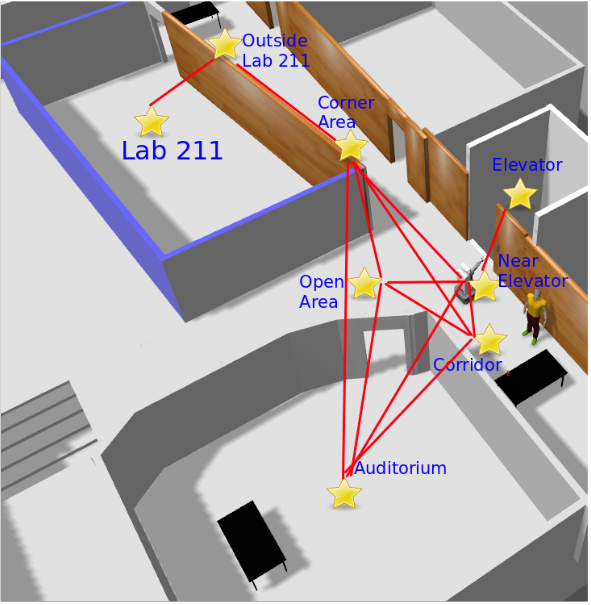
\includegraphics[width=.8 \linewidth]{PLP-Verify-ICAPS-2021/floor-layout.png}
%  \caption{Floor Layout: ``stars” are the locations the robot can navigate between.}
%  \label{fig:robotic-example-floor-layout}
%\end{figure}

\begin{figure*}[htb!]
  \centering
  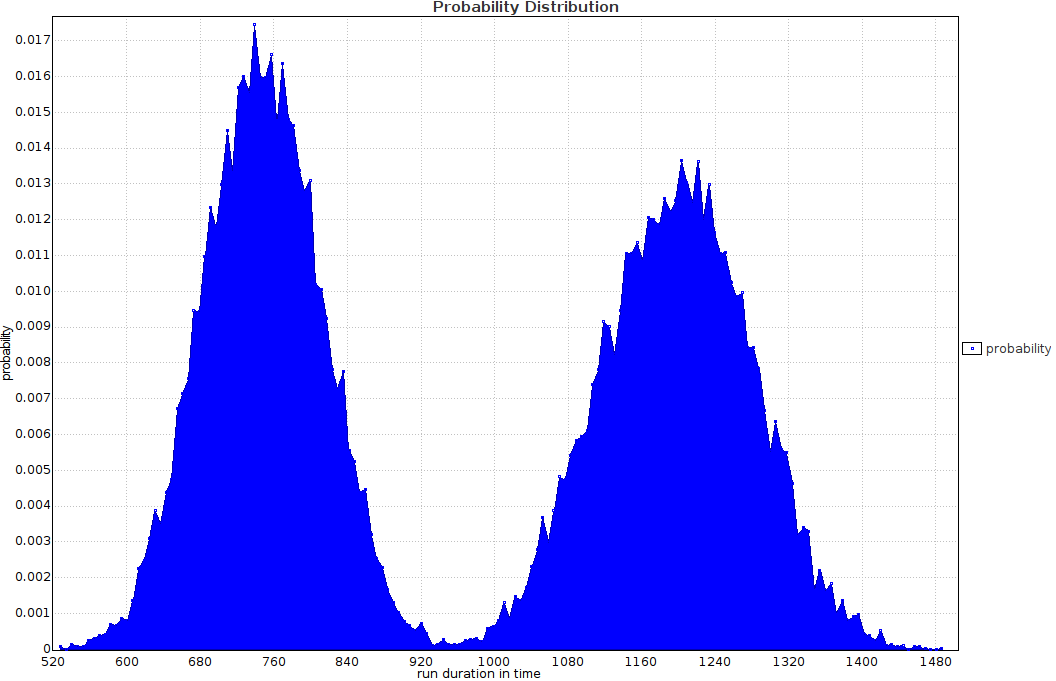
\includegraphics[width=.66\linewidth]{PLP-Verify-ICAPS-2021/Q1-1_prob_dist.png}
  %removedVspace
  \caption{Run time distribution of the system for Query 1.}
  \label{fig:robotic-example-query1}
\end{figure*}

\begin{figure}
  \centering
  % include second image
  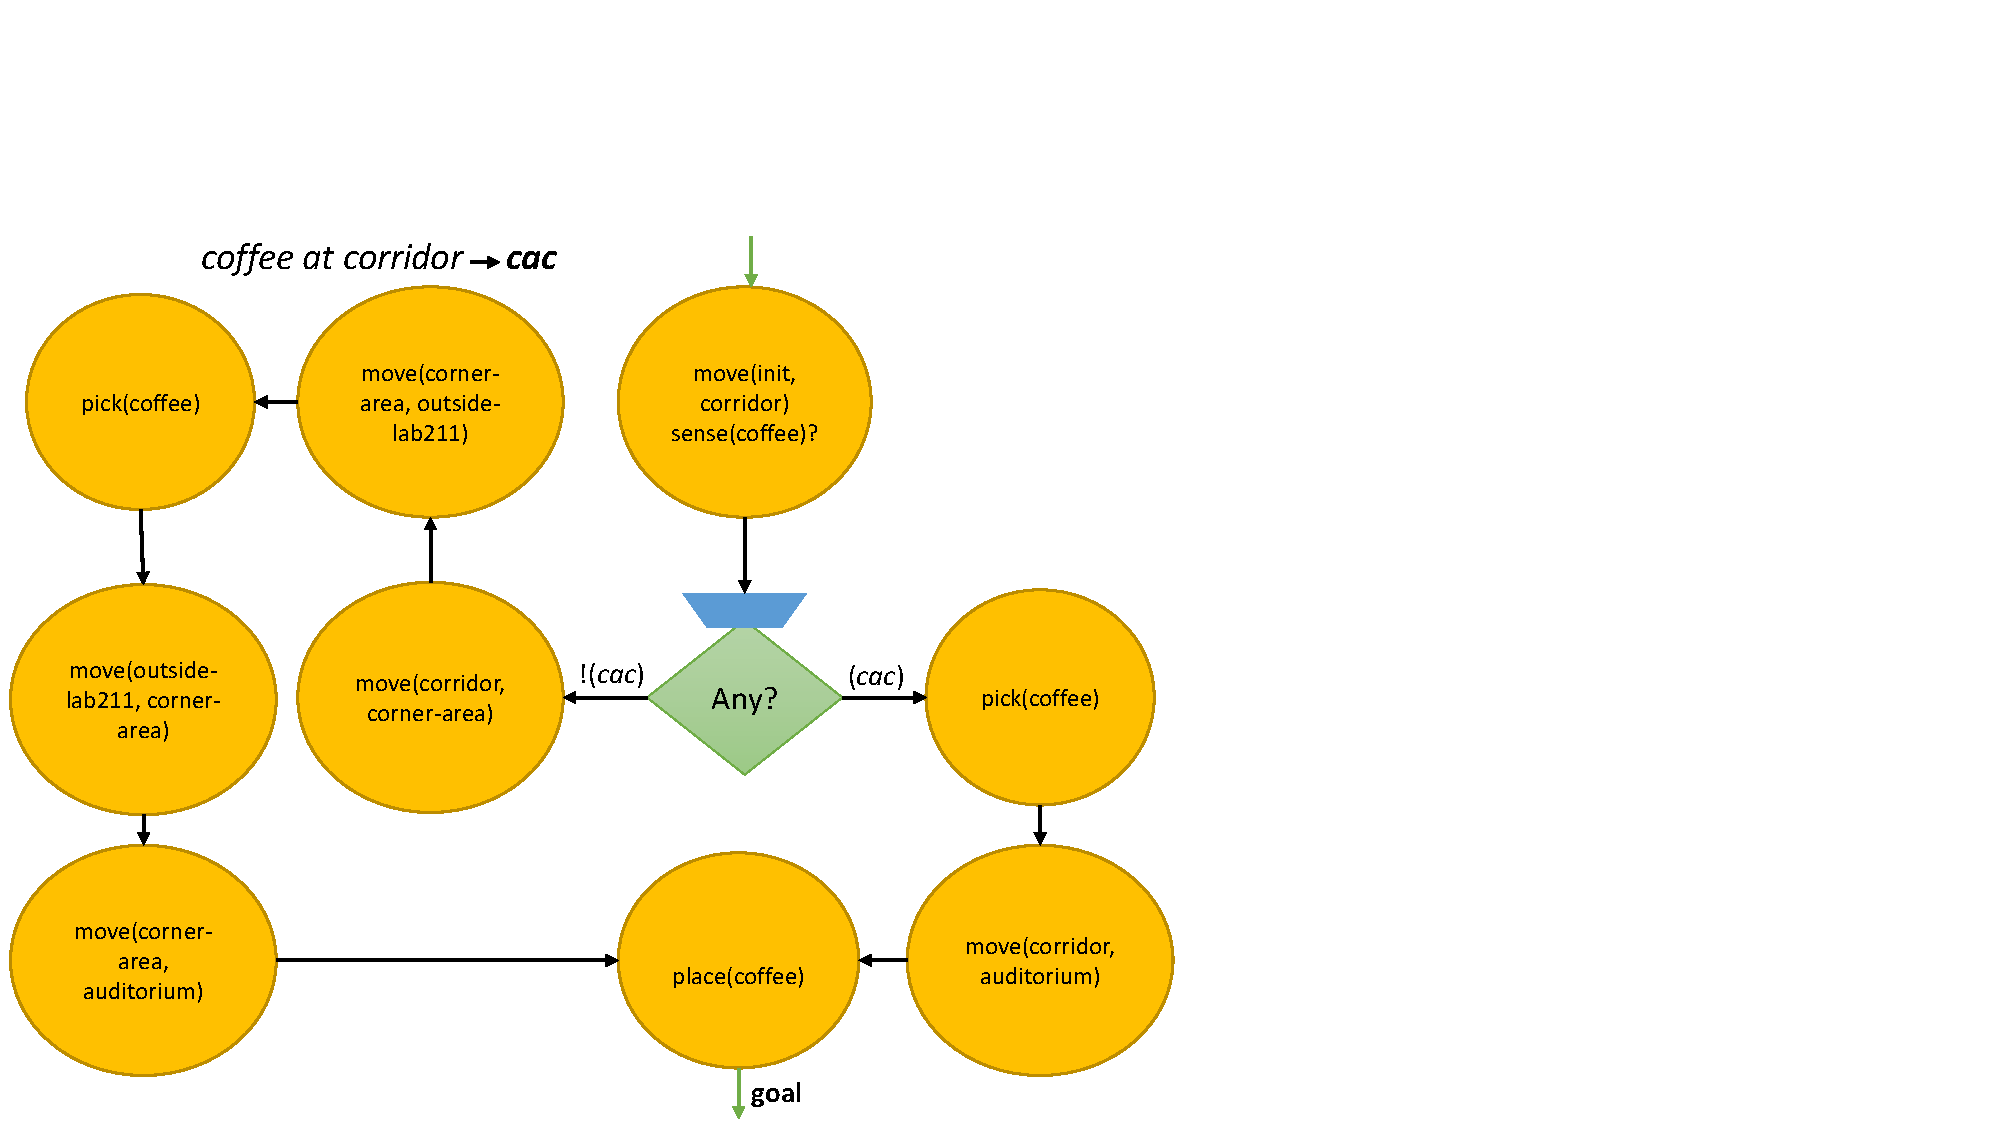
\includegraphics[width=.987\linewidth]{PLP-Verify-ICAPS-2021/example1ControlGraph-1-1.pdf}
  %removedVspace
  \caption{The control graph for the service robot example.}
  \label{fig:robotic-example-control-graph}
\end{figure}



% \begin{figure}
%   \centering
%   % include second image
%   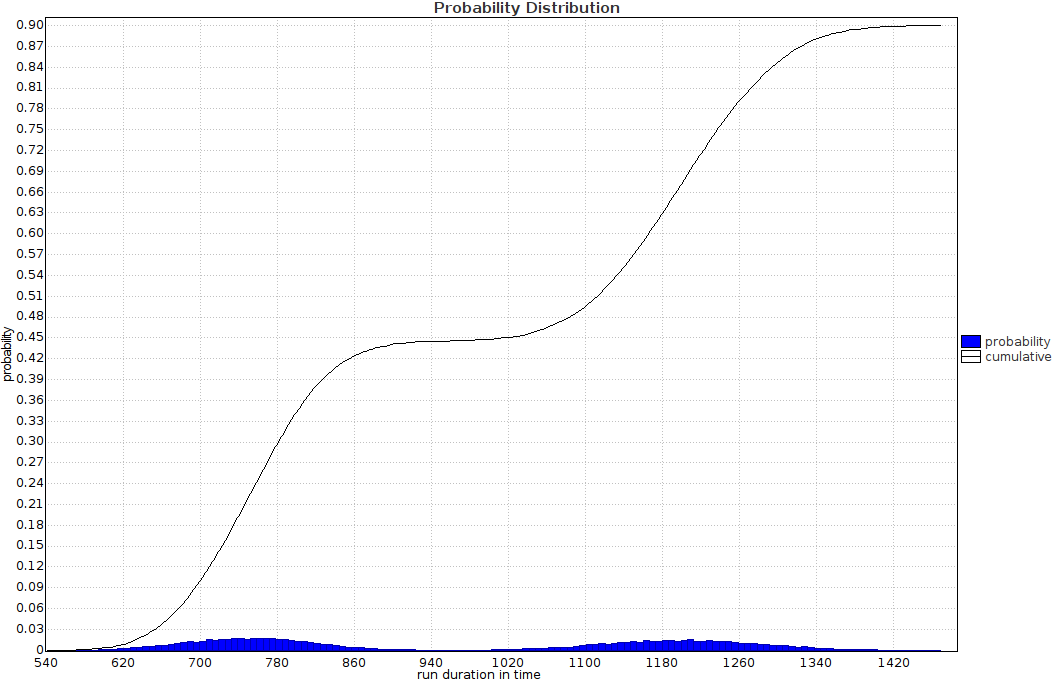
\includegraphics[width=.99 \linewidth]{PLP-Verify-ICAPS-2021/Q1-1_cumulative_prob_dist.png}
%   \caption{Run time distribution of the system for Query 2.}
%   \label{fig:robotic-example-query2}
% \end{figure}

%%%%%

\commentout{
%%%%%
\begin{figure*}[]
\centering
\begin{subfigure}{.46\textwidth}
  \centering
  % include first image
  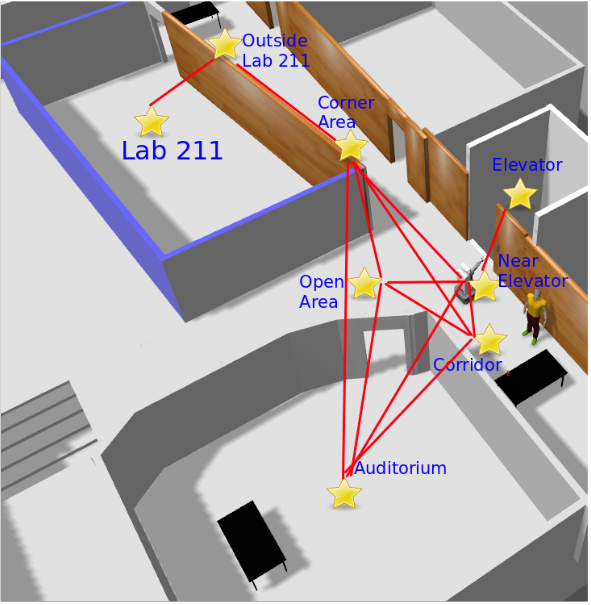
\includegraphics[width=.73 \linewidth]{PLP-Verify-ICAPS-2021/floor-layout.png}
  \caption{Floor Layout: ``stars” are the locations the robot can navigate between.}
  \label{fig:robotic-example-floor-layout}
\end{subfigure}
\hspace{0.1in}

\begin{subfigure}{.48\textwidth}
  \centering
  % include second image
  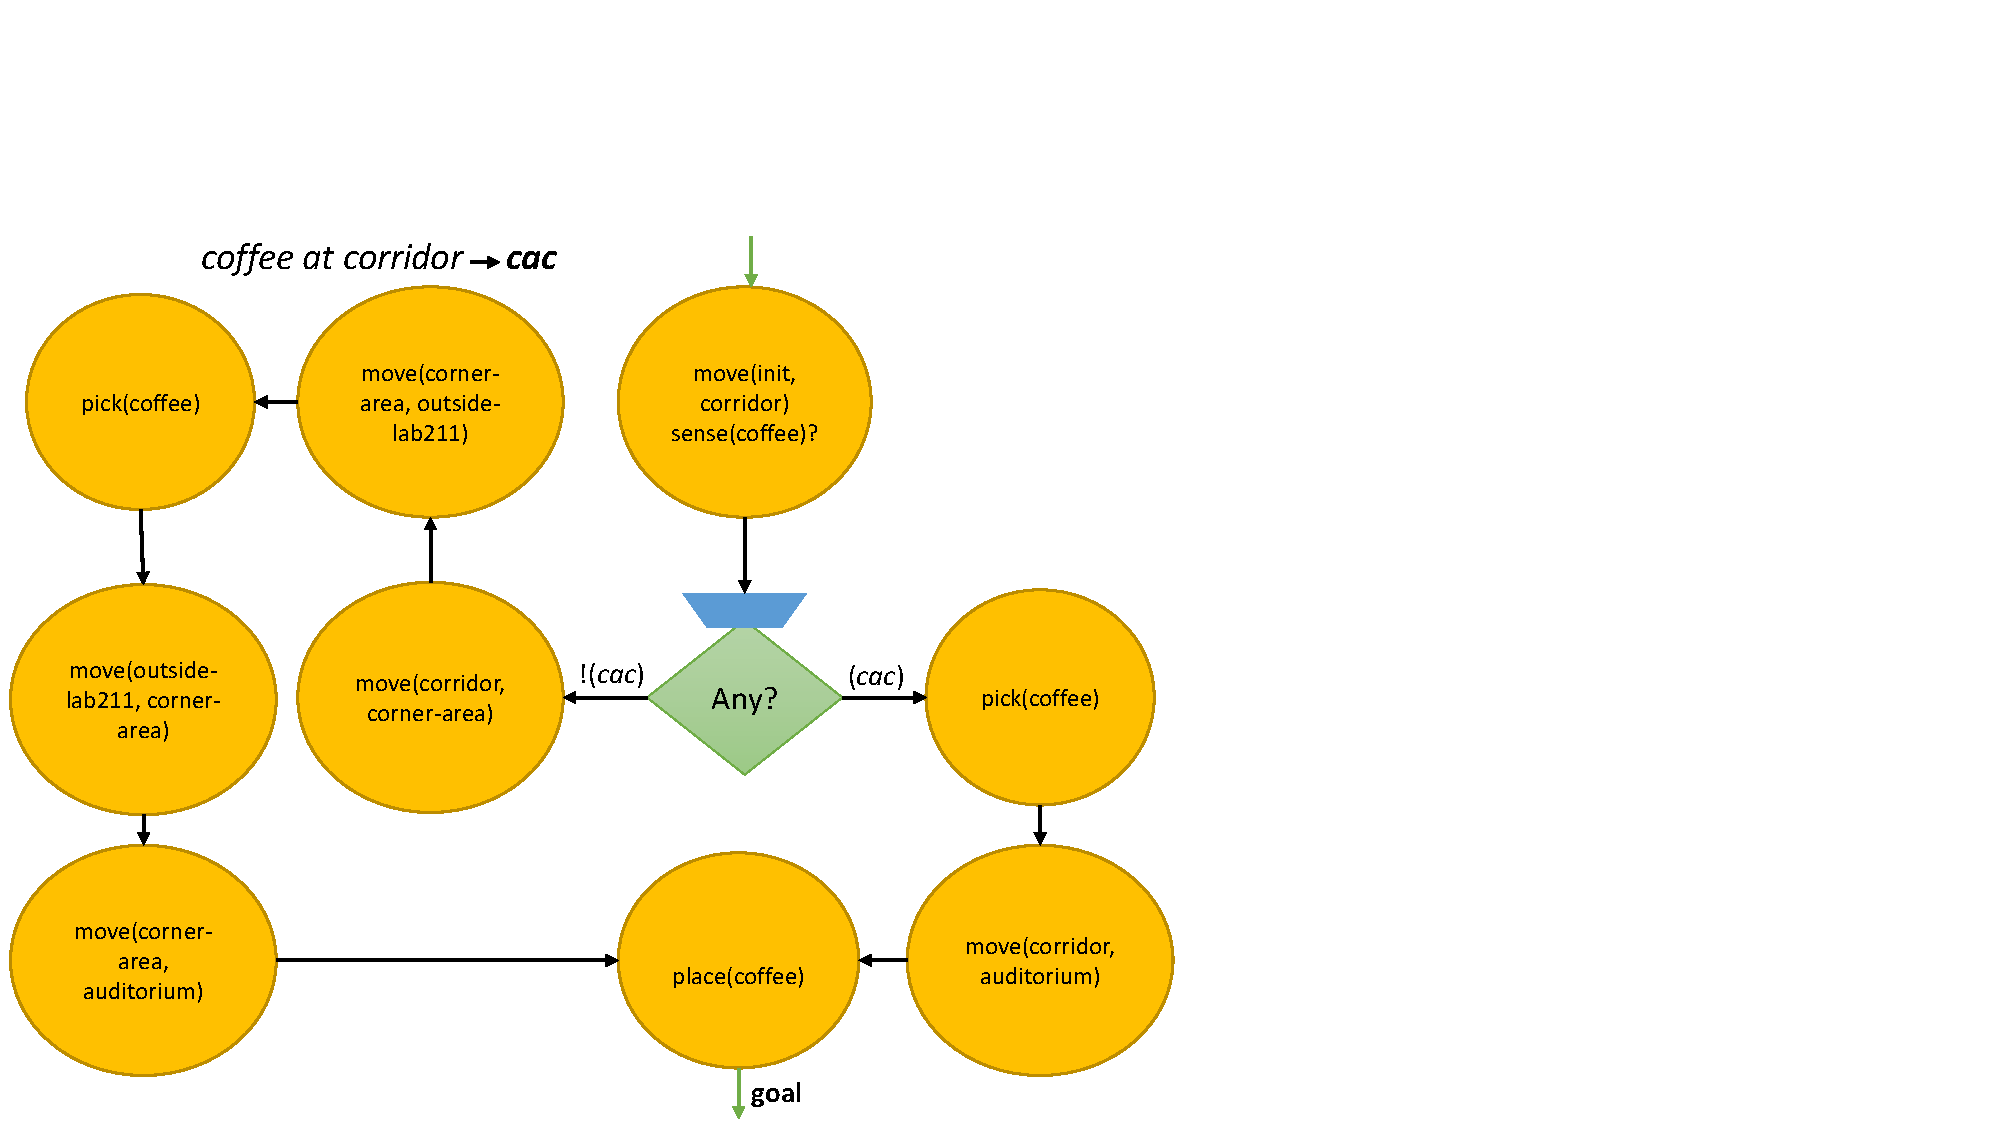
\includegraphics[width=.83\linewidth]{PLP-Verify-ICAPS-2021/example1ControlGraph-1-1.pdf}
  \caption{The control graph for the service robot example.}
  \label{fig:robotic-example-control-graph}
\end{subfigure}
%removedVspace

\begin{subfigure}{.48\textwidth}
  \centering
  % include first image
  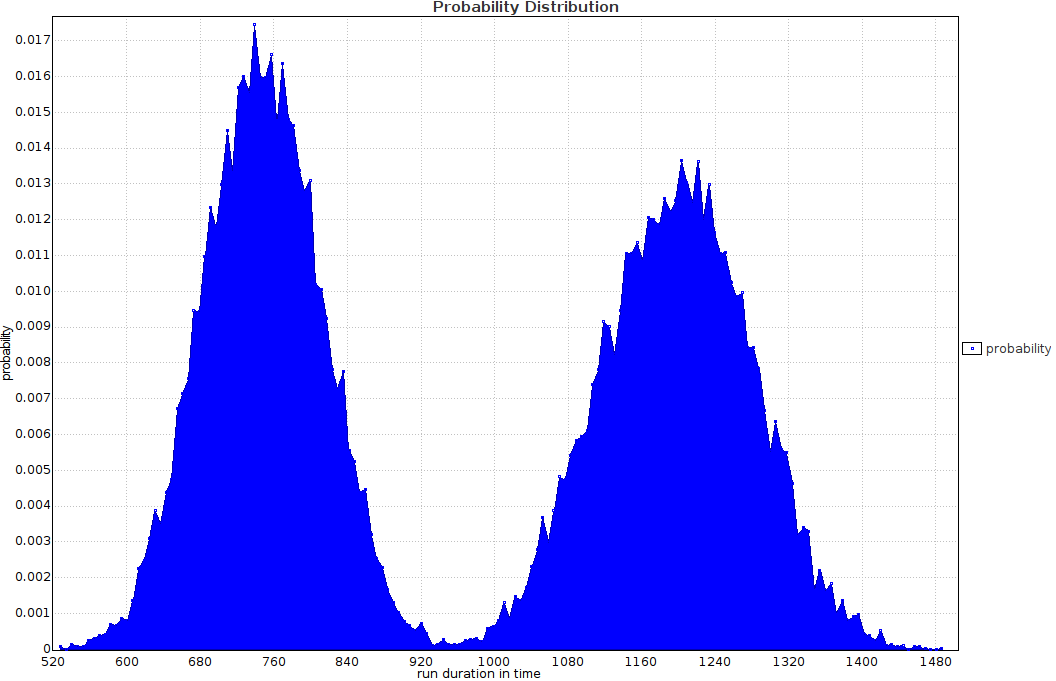
\includegraphics[width=.83\linewidth]{PLP-Verify-ICAPS-2021/Q1-1_prob_dist.png}
  \caption{Run time distribution of the system for Query 1.}
  \label{fig:robotic-example-query1}
\end{subfigure}
\hspace{0.1in}
\begin{subfigure}{.48\textwidth}
  \centering
  % include second image
  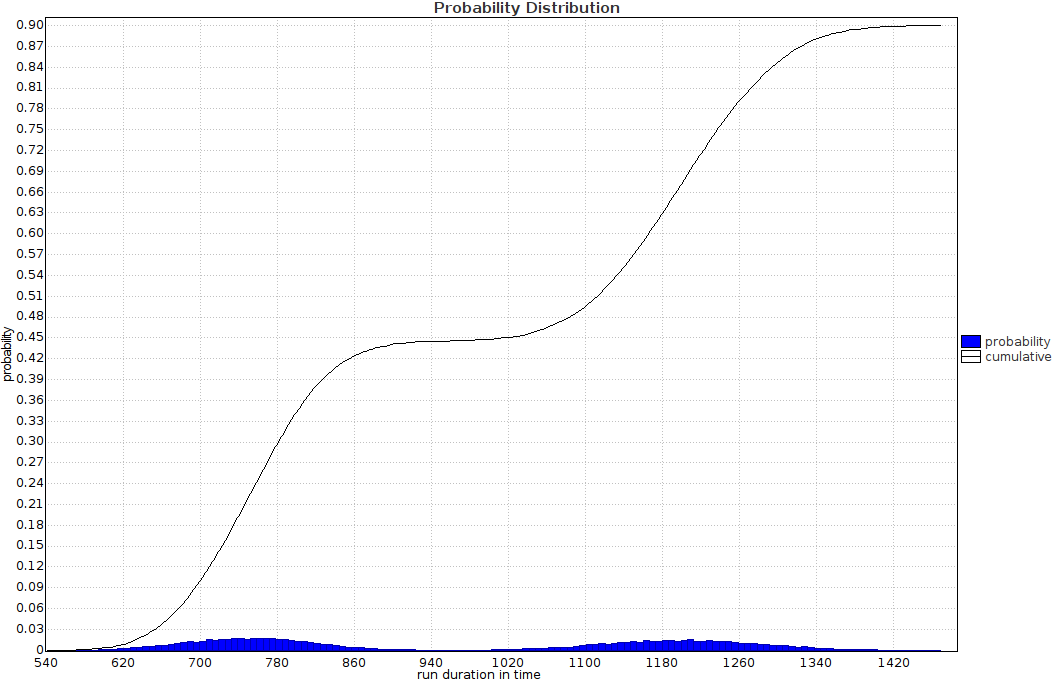
\includegraphics[width=.83 \linewidth]{PLP-Verify-ICAPS-2021/Q1-1_cumulative_prob_dist.png}
  \caption{Run time distribution of the system for Query 2.}
  \label{fig:robotic-example-query2}
\end{subfigure}
\caption{Case Study: The service robot example.}
\label{fig:robotic-example-queries}
\end{figure*}
%%%%%
}

The second query we tested was a probability (``$Pr<>$") query of successfully reaching the most distant PTA\textsubscript{PLP} from the initial state. We defined each PLP with one failure and one success path, both with certain probabilities. UPPAAL calculates probability by multiple evaluations (i.e., by sampling runs), which may take a long time.
%
% \begin{figure}[t]
% \centering
% %%removedVspace
% \includegraphics[scale=0.3]{chartQueryProbabilisticDuration.png}
% %%removedVspace
% \caption{Average Time for Probability Query}
% \label{fig:prob-time}
% %removedVspace
% \end{figure}
%
%
% \begin{figure}[t]
% \centering
% %%removedVspace
% \includegraphics[scale=0.3]{chartQueryProbabilisticRAM.png}
% %%removedVspace
% \caption{Avg. RAM Consumed for Prob. Query}
% \label{fig:prob-memory}
% %removedVspace
% \end{figure}
%
%
The results are show in Figure~\ref{fig:time-prob-query}. %and~\ref{fig:ram-prob-query}.
%~\ref{fig:prob-time} and~\ref{fig:prob-memory}.
%\frameImage{chartQueryProbabilisticDuration.png}{1.8in}{2.6in}{Average probabilistic query duration}
%\frameImage{chartQueryProbabilisticRAM.png}{1.8in}{2.6in}{Average RAM consumed by probabilistic query}
Again, we see that query time for smaller models is reasonable. Certainly, verifying controller properties off-line is realistic, and on, e.g., a service robot operating in the home environment without severe time pressure, online evaluation is possible, too.

% \begin{figure}
%     \centering
%     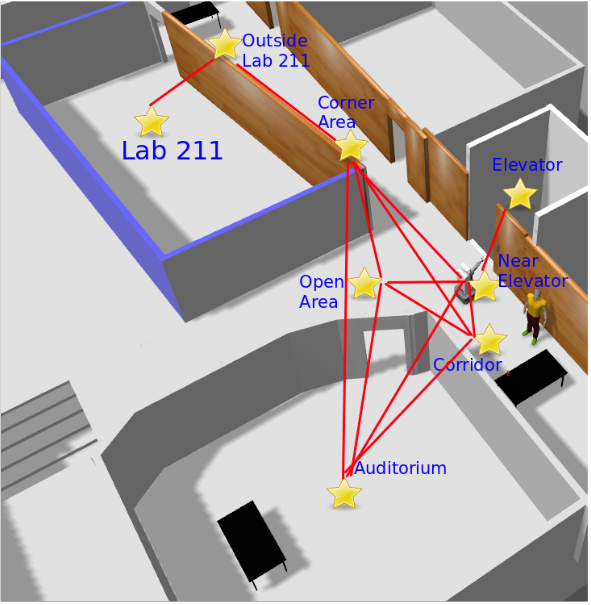
\includegraphics[scale=0.4]{PLP-Verify-ICAPS-2021/floor-layout.png}
%     \caption{Floor Layout: ``stars" denote possible locations the robot can navigate between.}
%     %two connected locations -- shown by red lines.}
%     \label{fig:floor-layout}
% \end{figure}

% \begin{figure*}[ht]
% \centering
% \begin{subfigure}{.35\textwidth}
%   \centering
%   % include first image
%   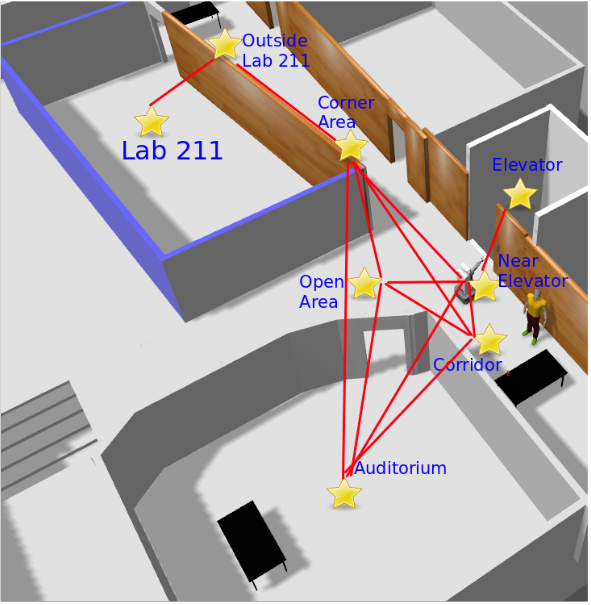
\includegraphics[width=.98\linewidth]{PLP-Verify-ICAPS-2021/floor-layout.png}
%   \caption{Floor Layout: ``stars” denote possible locations the robot can navigate between.}
%   \label{fig:robotic-example-floor-layout}
% \end{subfigure}
% %%removedVspace

% \begin{subfigure}{.35\textwidth}
%   \centering
%   % include second image
%   \includegraphics[width=.98\linewidth]{PLP-Verify-ICAPS-2021/control-greaph-armadillo.png}
%   \caption{The control graph for the service robot example.}
%   \label{fig:robotic-example-control-graph}
% \end{subfigure}
% % \caption{The service robot example case study.}

% % \label{fig:robotic-example}
% % \end{figure*}
% %\newline
% %removedVspace

% % \begin{figure}[hbt!]
% % \centering
% \begin{subfigure}{.35\textwidth}
%   \centering
%   % include first image
%   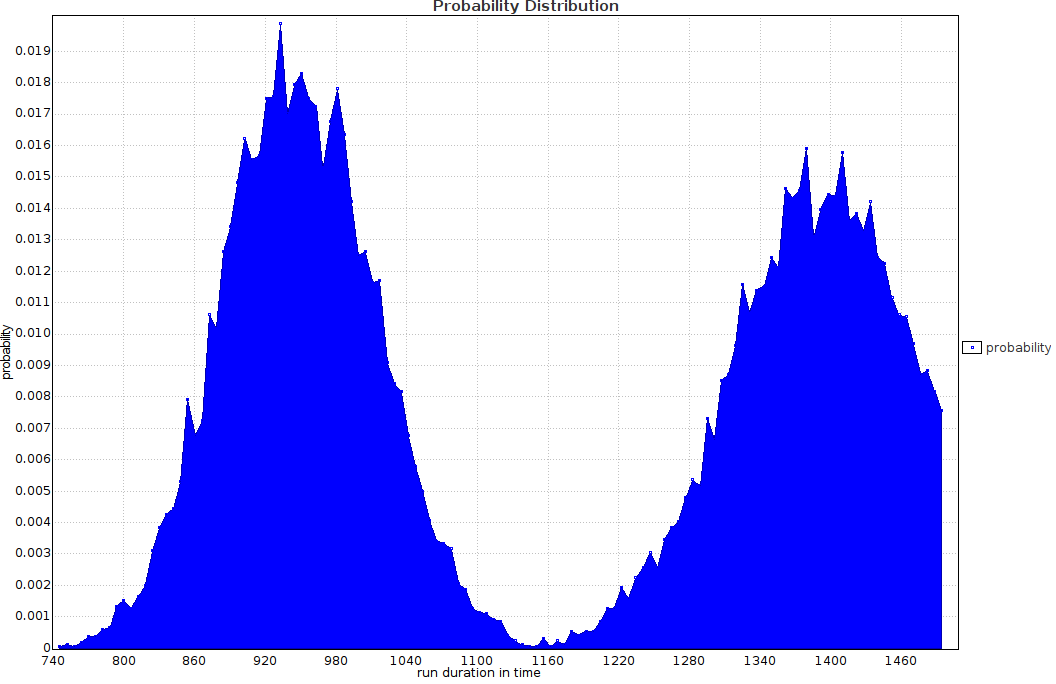
\includegraphics[width=.98\linewidth]{PLP-Verify-ICAPS-2021/Q1-2_prob_dist.png}
%   \caption{Run time distribution of the system for Query 1.}
%   \label{fig:robotic-example-query1}
% \end{subfigure}
% %%removedVspace

% \begin{subfigure}{.35\textwidth}
%   \centering
%   % include second image
%   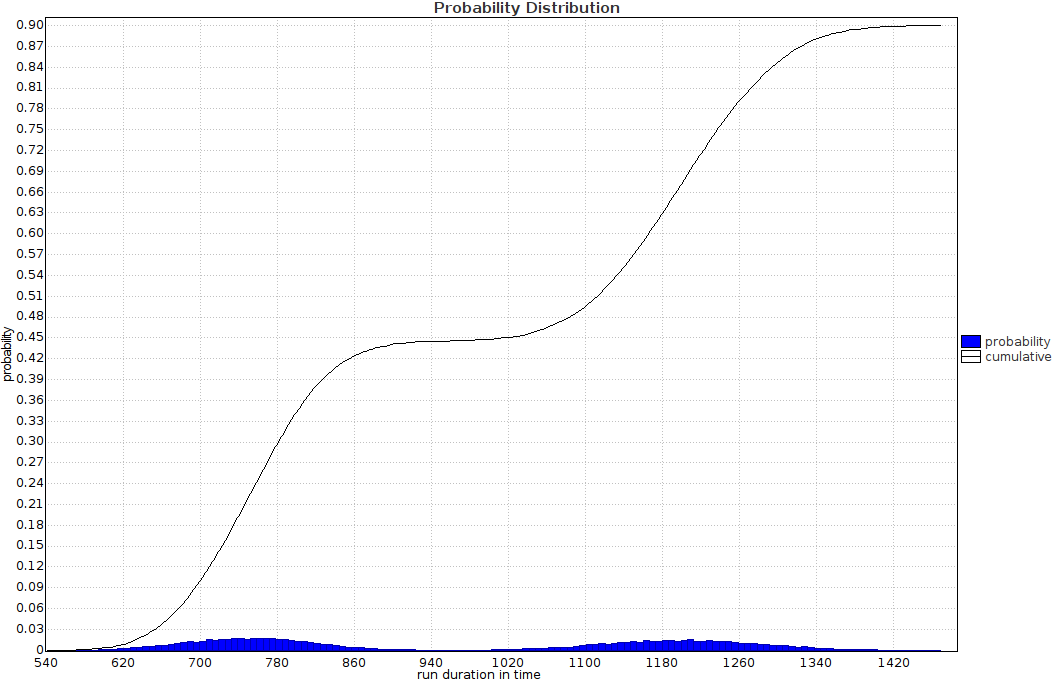
\includegraphics[width=.98\linewidth]{PLP-Verify-ICAPS-2021/Q1-1_cumulative_prob_dist.png}
%   \caption{Run time distribution of the system for Query 2.}
%   \label{fig:robotic-example-query2}
% \end{subfigure}
% \caption{The service robot example case study.}
% \label{fig:robotic-example-queries}
% \end{figure*}


\noindent{\bf Service Robot Case Study.}\ \
Next, we evaluated our system on a simulated real-world scenario.
%In a real world scenario,
ARMadillo -- a service robot at our lab, is to serve coffee to a person in the auditorium.
%Floor layout is shown in  Figure~\ref{fig:robotic-example-floor-layout} and
The robot's possible actions are {\em observe} coffee cup, {\em navigate} to different locations at our office floor, and {\em pick} and {\em place}. %respectively, to pick the coffee cup and deliver it to the person by placing the cup on the table in the auditorium.
%
%
%
%
% \begin{figure}
%     \centering
%     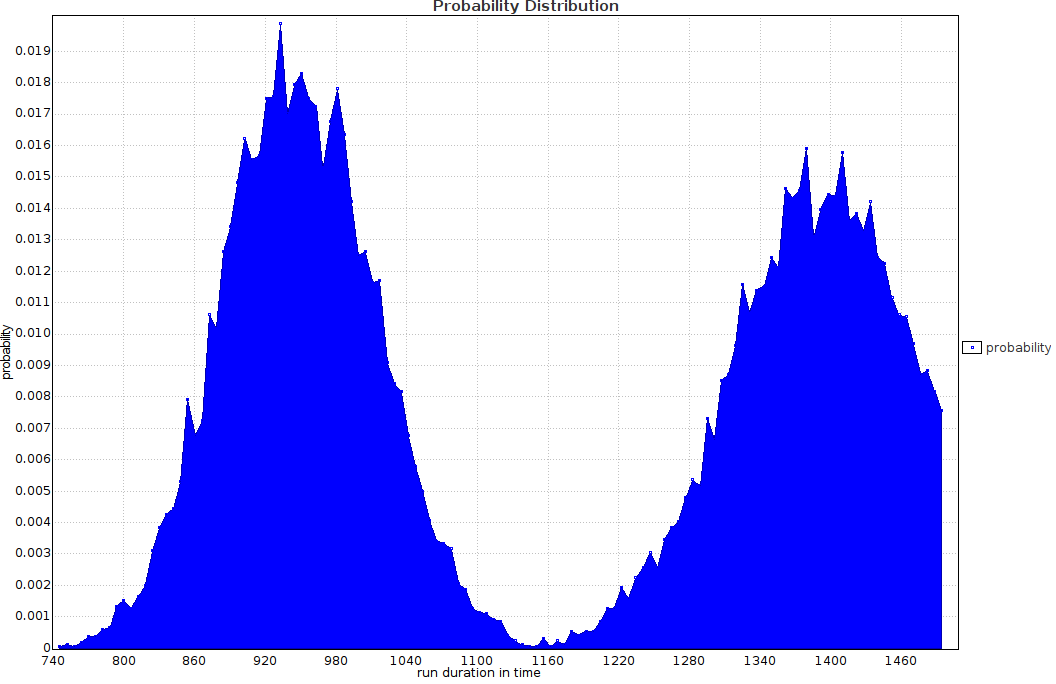
\includegraphics[scale=0.3]{PLP-Verify-ICAPS-2021/Q1-2_prob_dist.png}
%     \caption{Run time distribution of the system for Query 1.}
%     \label{fig:Q1-2-pd}
% \end{figure}
%
% \begin{figure}
%     \centering
%     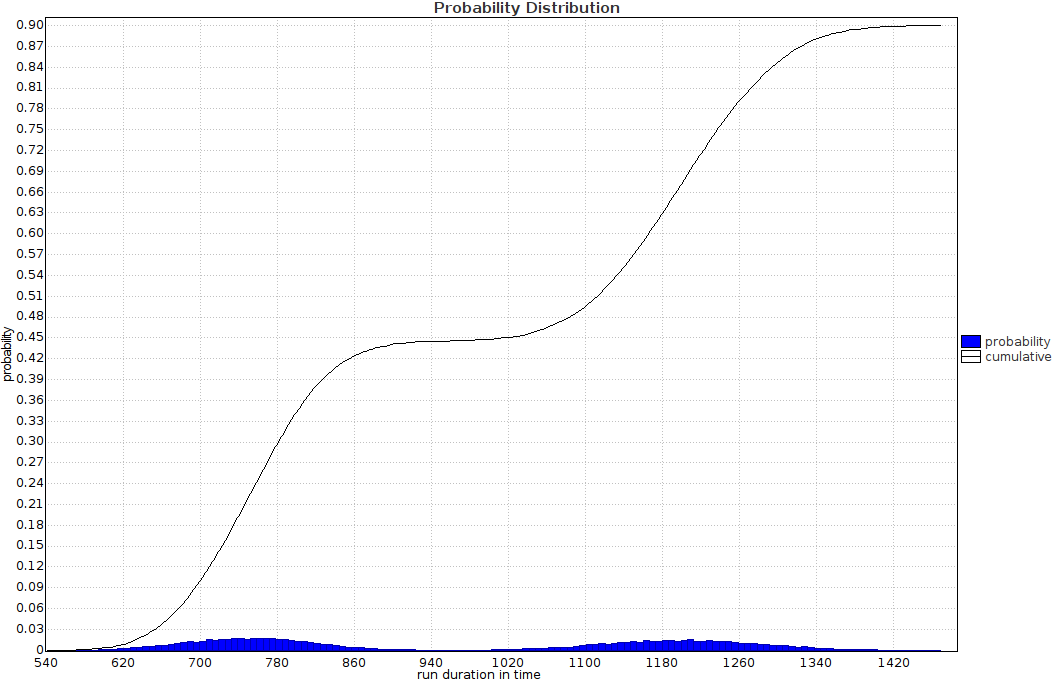
\includegraphics[scale=0.3]{PLP-Verify-ICAPS-2021/Q1-1_cumulative_prob_dist.png}
%     \caption{Run time distribution of the system for Query 2.}
%     \label{fig:Q1-1-cpd}
% \end{figure}
%
The robot starts near the elevator and the coffee is either at corridor area or outside lab211. Its control graph is shown in Figure~\ref{fig:robotic-example-control-graph}.
%Two runs of this simulations can be found in \url{https://youtu.be/2DjMdOZUruk} and  \url{https://youtu.be/w3F5vhDF6oI}.
The robot executes an {\em achieve} PLP, followed by an {\em observe} PLP, followed by a {\em conditional node} that branches into  two sequences of {\em achieve} PLPs.
%Based on this, we created two possible worlds in the Gazebo simulation such that they are identical except for, in World 1 the coffee cup appears on the table in the corridor area, while in World 2, the cup appears on the table in outside lab211 area.
%Demos for these possible worlds are shown in the following YouTube videos. For World 1: \url{https://youtu.be/2DjMdOZUruk} and for World 2: \url{https://youtu.be/w3F5vhDF6oI}. Each demo basically tests the ability of a ROS based online POMDP planner to effectively find appropriate actions online, receive observations, perform appropriate belief update, and achieve its goal. Figure~\ref{fig:online-execution-demo-screenshot} shows the robot carrying coffee and entering auditorium to serve it to the person.



%\begin{figure}
%    \centering
%    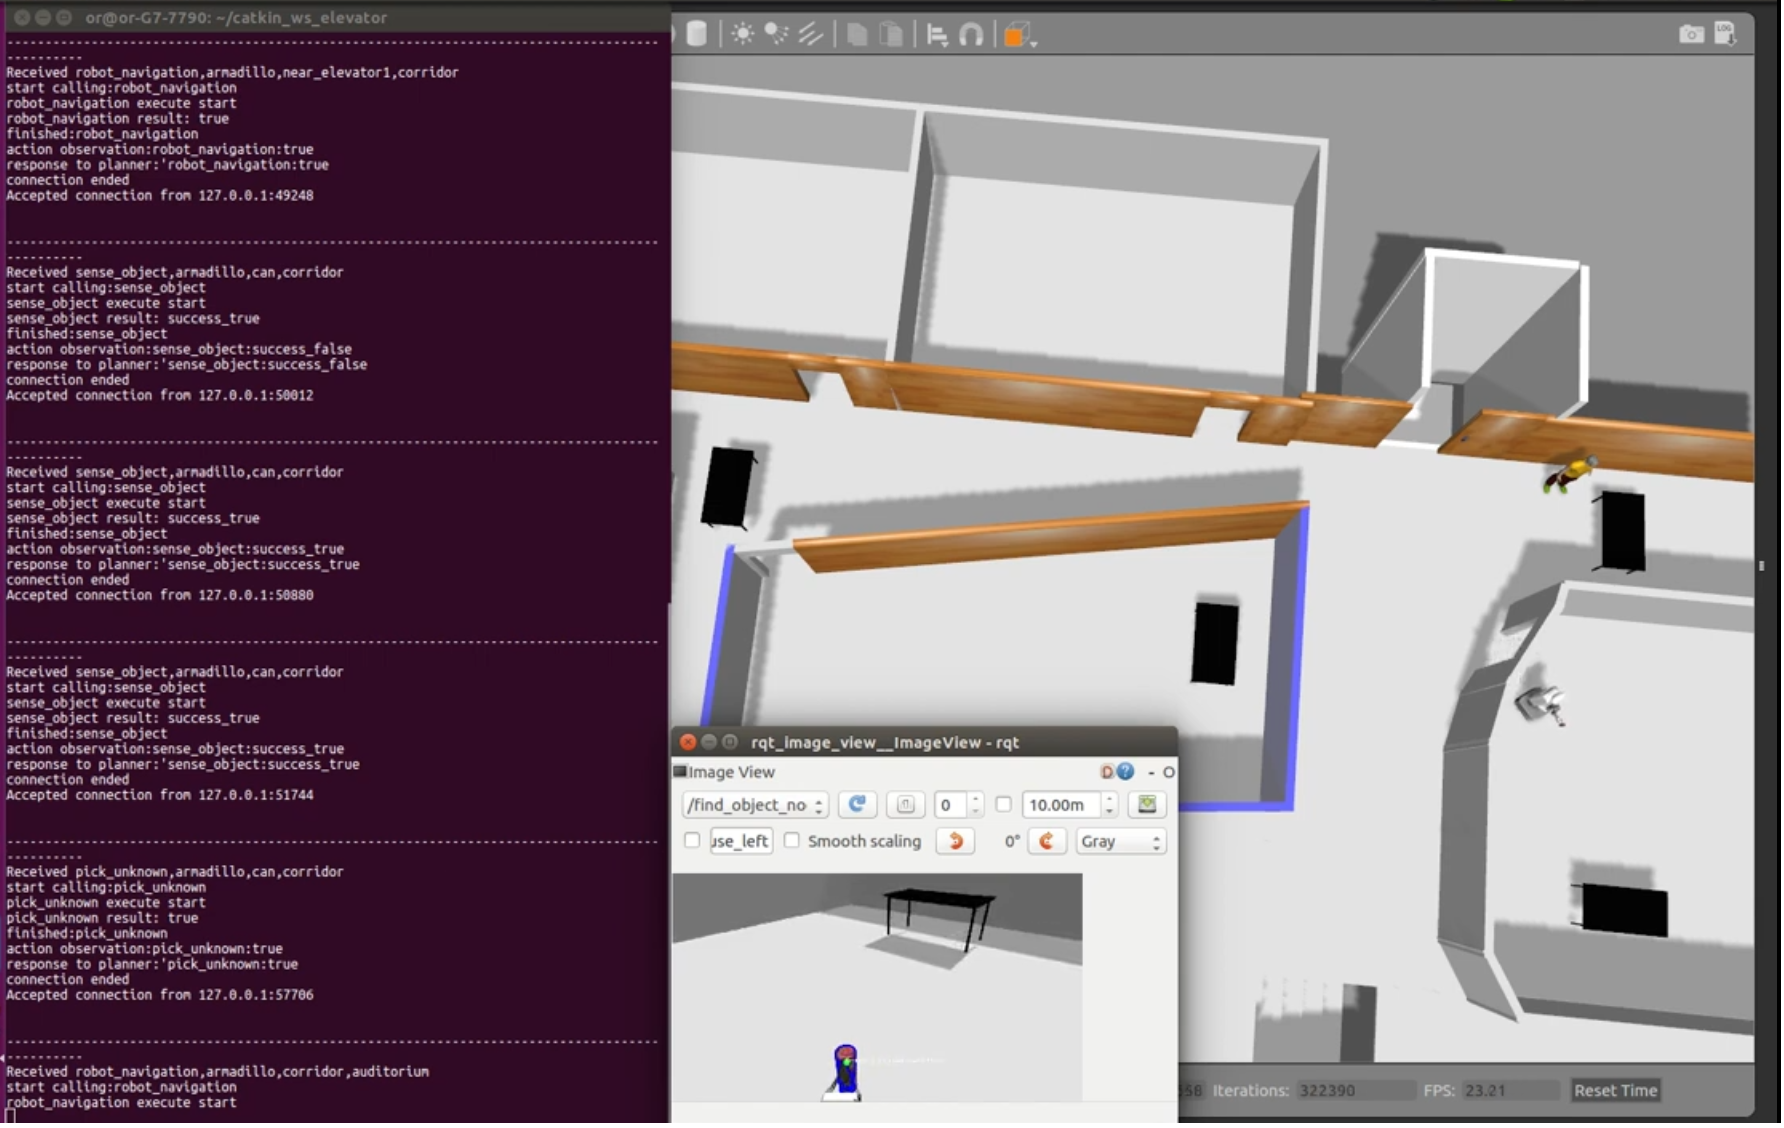
\includegraphics[scale=0.21]{PLP-Verify-ICAPS-2021/robot moving towards auditorium holding coffee.png}
%    \caption{Robot enters auditorium to deliver coffee.}% to the person.}
%    \label{fig:online-execution-demo-screenshot}
%\end{figure}

%The third test case is based on the service robot example, which takes a middle route, i.e., it is not as complex to compile as the first test case but more complex than the second test case.
%We considered the example scenario.
%Based on the demos, we created a complete offline plan tree keeping the two possible worlds under consideration.
%This plan tree helps generate a control graph for the scenario as shown in Figure~\ref{fig:robot-example-cg}.


% \begin{figure}
%     \centering
%     \includegraphics[scale=0.25]{control-greaph-armadillo.png}
%     \caption{The control graph for the service robot example. }
%     \label{fig:robot-example-cg}
% \end{figure}

We compiled the control graph and the PLPs for the demo's code into an UPPAAL input file.
We assumed all the actions eventually succeed, except for the {\em place} action that fails with probability 0.1.
%Here we show the results
%of the natural query: will we get the coffee
%as per the required input format), and produced a single file for UPPAAL.
Query 1 asks for the probability that the person will get the coffee before it gets cold, where we used 25 minutes as the time limit. %arbitrarily set the time
%We tested the system's properties with the help of several UPPAAL queries. For example, Query 1 is ``What is the probability of the person being served in the next 25 minutes from now?"
The output generated is a probability range [0.895, 0.90] with confidence of 99.5\%.  Figure~\ref{fig:robotic-example-query1} describes the PDF over this time steps, showing two peaks -- one for each path of the control graph.
The query took 15.15 seconds and 56.2 Mb of memory.
If we reduce the time limit to 20 minutes, then the probability range drops to [0.67, 0.68] with confidence of 99.5\%.
This query took 34.36 seconds and 56.7 Mb of memory.
Query 2 asked what is the probability that the coffee will ultimately be served? %(Cumulative) Probability Distribution for Query 2 --- ``What is probability that in each path eventually the coffee will be served?" is
UPPAAL took 11.72 seconds and 47.1 Mb of memory to return the probability range [0.896, 0.905] with a confidence of 95\% within 100 thousands time units (i.e., $\mathrm{Pr[\leq 100000] (<> ...)}$).
%The PDF is shown in Figure~\ref{fig:robotic-example-query2}.
%Note that the overall resources required to verify a query depends on that query itself, along with the number of paths (and their lengths) need to be evaluated, as well as the properties of PTAs graph.
%\shashank{ end}



%%%%%%
\commentout{
\section{Online Monitoring and Learning With PLPs}
\subsection{Code Generation for Monitoring}
Given a PLP file, we can automatically generate code for a ROS package %containing a single node
that monitors the performance of the module when executed.%
\footnote{We do not support code generation for {\em repeat\/} constructs, yet.}
%While generating the harness node,
To map PLP parameters to their location in ROS (e.g., the topic) we use
a \textit{glue} file. The glue file also contains the required imports in order to work with the needed messages and classes.

This generated ROS package performs the following functionality: The PLP Harness saves the most recent value of each parameter as referred to by the given glue file. Each time a value is updated, the PLP Harness checks whether the PLP trigger holds (start condition). When it does, the harness node creates a PLP object. The newly created PLP object is updated whenever one of its parameters are updated, and uses the harness to publish alerts and predictions regarding the task it monitors. In particular, we can get alerts when preconditions, concurrency conditions, progress measures or other required conditions are violated, and we can receive updated predictions regarding the success probability and expected execution time.
%This code can also collect statistics online regarding success and failure probabilities, as well as run-time distributions.
Thanks to a clear distinction between the ROS node and the PLP logic we can adapt to support platforms other than ROS.
%also use the PLPs in off-line contexts, such as planning.

There are two main parts that are left as ``templates" for the programmer to implement: 1. Variable updaters -- when a parameter is updated, the methods for recalculating the variables will be called. These functions must be filled in by the user. 2. Condition validation functions -- each function checks if some basic condition specified somewhere in the PLP holds. The user is asked to fill in code that validates only the bare essential conditions.
Each of these functions is generated with comments describing what needs to be implemented in a clear and simple manner.


%An event diagram for the PLP object is shown in Figure~\ref{fig:event-diagram}.

%\begin{figure}[t]
%\centering
%%removedVspace
%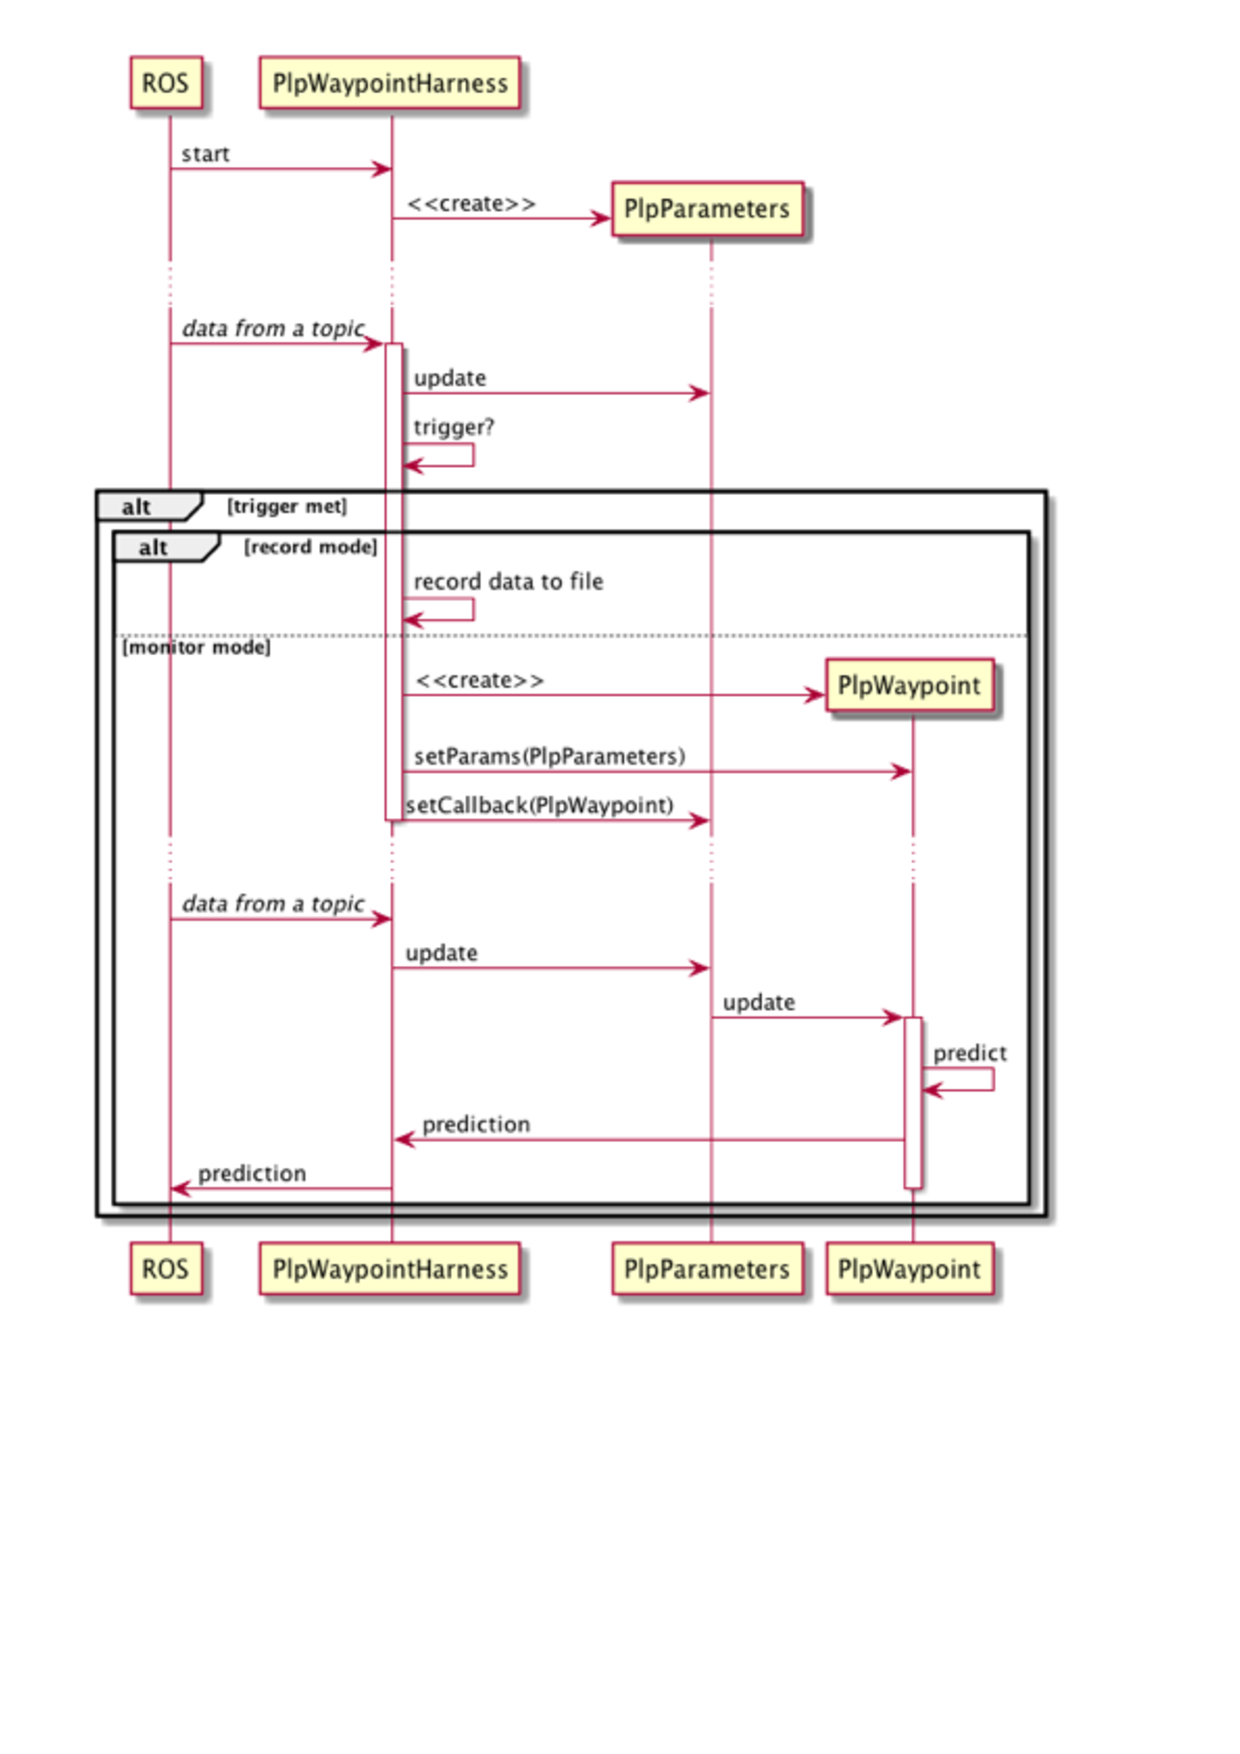
\includegraphics[scale=0.3]{code-generation}
%%removedVspace
%\caption{Event Diagram for PLP Generate Code}
%\label{fig:event-diagram}
%%removedVspace
%\end{figure}

\subsection{Code Generation for Data Gathering}
An important component of the PLP is a statistical profile of some of its properties, such as success rate and run-time distribution.
%and more ROS specific statistics, such as the rate in which messages are published or read.
 Our statistics collecting code is generated automatically from a PLP and is, in fact,
%works initially very much like the PLP code does. In fact,
an operating mode of the aforementioned ROS harness node. When started in ``data gathering mode", the ROS harness node records the parameters when the PLP's trigger condition becomes true. This allows for the following technique: run multiple simulations of a given task, with the ROS harness in data gathering mode. For each iteration, in addition to the file generated by the ROS harness node, record the final result (success, failure mode, run-time distribution, etc.). Next, compute statistics on this data -- at present averages for run-time and success probability and invariants, and automatically update the PLP file with this information.
%\subsection{Evaluation}


\section{ROS-BASED PLP TOOLS}
We developed three tools for defining and exploiting PLPs:
a PLP editor, automated code generation for run-time monitoring,
automated data analysis and PLP update, which we now briefly describe.
\begin{enumerate}
\item {\bf The PLP Editor.}
This is a dedicated editor for PLPs with standard features. While, in principle, due to our definition of XSDs for each PLP type, any XML editor could be used, using a dedicated tool, we are able to support  add-ons, and also to make the PLP definition easier. In particular, an important element in the use of PLPs is relating the formal parameters with ROS topics, and our tool provides support for this and automatically creates the glue file.

\item {\bf Monitoring Code Generation.} This tool creates
ROS monitoring code semi-automatically: monitoring preconditions, concurrency conditions, progress measures, and run-time, as described earlier.

\item {\bf PLP Statistics Profiler.}
This tool updates the PLP with information gathered during run-time.
This includes statistical information about run-time and success, with the possibility of allowing automated update of the relevant fields in the PLP.
\end{enumerate}
In addition, we  developed a method for detecting a rich set of invariants, automatically~\citep{MatanThesis}. The software developed for it updates the invariant field of the relevant PLP.%
\footnote{Automated monitoring code generation for invariants is not supported yet, as it requires computing temporal features online. We are currently working on efficient online computation of these features.}
} %end commnetout




%endsection{Control Graph Verifier}
%\subsection{Play-outs and Planning}
%PLPs can be used for predicting the behavior of modules, and in particular, the behavior of module combinations, such as modules that run in sequence or in parallel, or in a loop. This calls for a theory of PLP composition, which is the subject of ongoing work. At present, we are focusing
%on predicting the success probability and run-time distribution of a set of PLP, run in sequence and in parallel
%Initial results on the complexity of exact and approximate computation of the success probability and run-time distribution for combinations
%of sequence and parallel execution of code associated with PLPs have been obtained (with exact computation being NP-hard, typically,
%and polytime approximation algorithms)~\citep{LiatMSC}
%For more complex settings, we use Monte-Carlo simulations. A tool for automatically computing these statistics is now implemented within the
%autonomous bob-cat project. At certain points, an operator may intervene, providing the bob-cat with a certain sequences of actions to perform.
%Using the PLPs of the component actions, our tool is able to predict the success probability and run-time distribution of the sequence.
%In difference to earlier work such as~\citep{Lesire11} which attempts to predict worst-case behavior, we are attempting to estimate distributions over running times, or their moments.

\commentout{
\section{USE METHODOLOGY AND USE CASES}
Our suggested methodology of use for PLPs is described in Figure~\ref{fig:methodology}.
A PLP can optionally be used instead, or in addition to traditional specification languages by the system architect. By using a PLP, she is required to
provide more precise, quantifiable requirements, possibly providing more guidance to the programmer.
For example, if the specified expected success rate of the grasping module is high, the programmer may want to update the trajectory of the arm during its
motion based on input from the gripper camera. Next, the code is written, and a PLP describing its expected properties is defined (or modified, if
defined earlier). Then, using automated code generation, data-gathering code is generated and integrated into the ROS package. Whenever
the module executes, it triggers the measurement of various run-time and success statistics. This information is gathered over multiple runs
and is used to improve the PLPs itself.
%\footnote{Currently, it learns the run-time distribution and success probability. We intend to build richer statistical profile in the future.}
%The statistics gathered are used
%to update the predictive analysis carried out by the PLP object.
Next, given the PLP, one can use the automated code generator to generate monitoring code.
The generated code works online, monitoring the module's behavior and/or gathering statistics.
%that checks various properties at run-time.
%As software generation is typically an incremental process,
If the code changes, one can edit the
%none may learn new information about the module, such as possible
%side-effects, failure modes, and additional required context conditions; or, for various reason, the code is changed, or optimized.
PLP to reflect such changes, and regenerate the code.
%and thanks to the automated code generation, the relevant software can be generated and used to replace the old version.

\begin{figure}[t]
\centering
%removedVspace
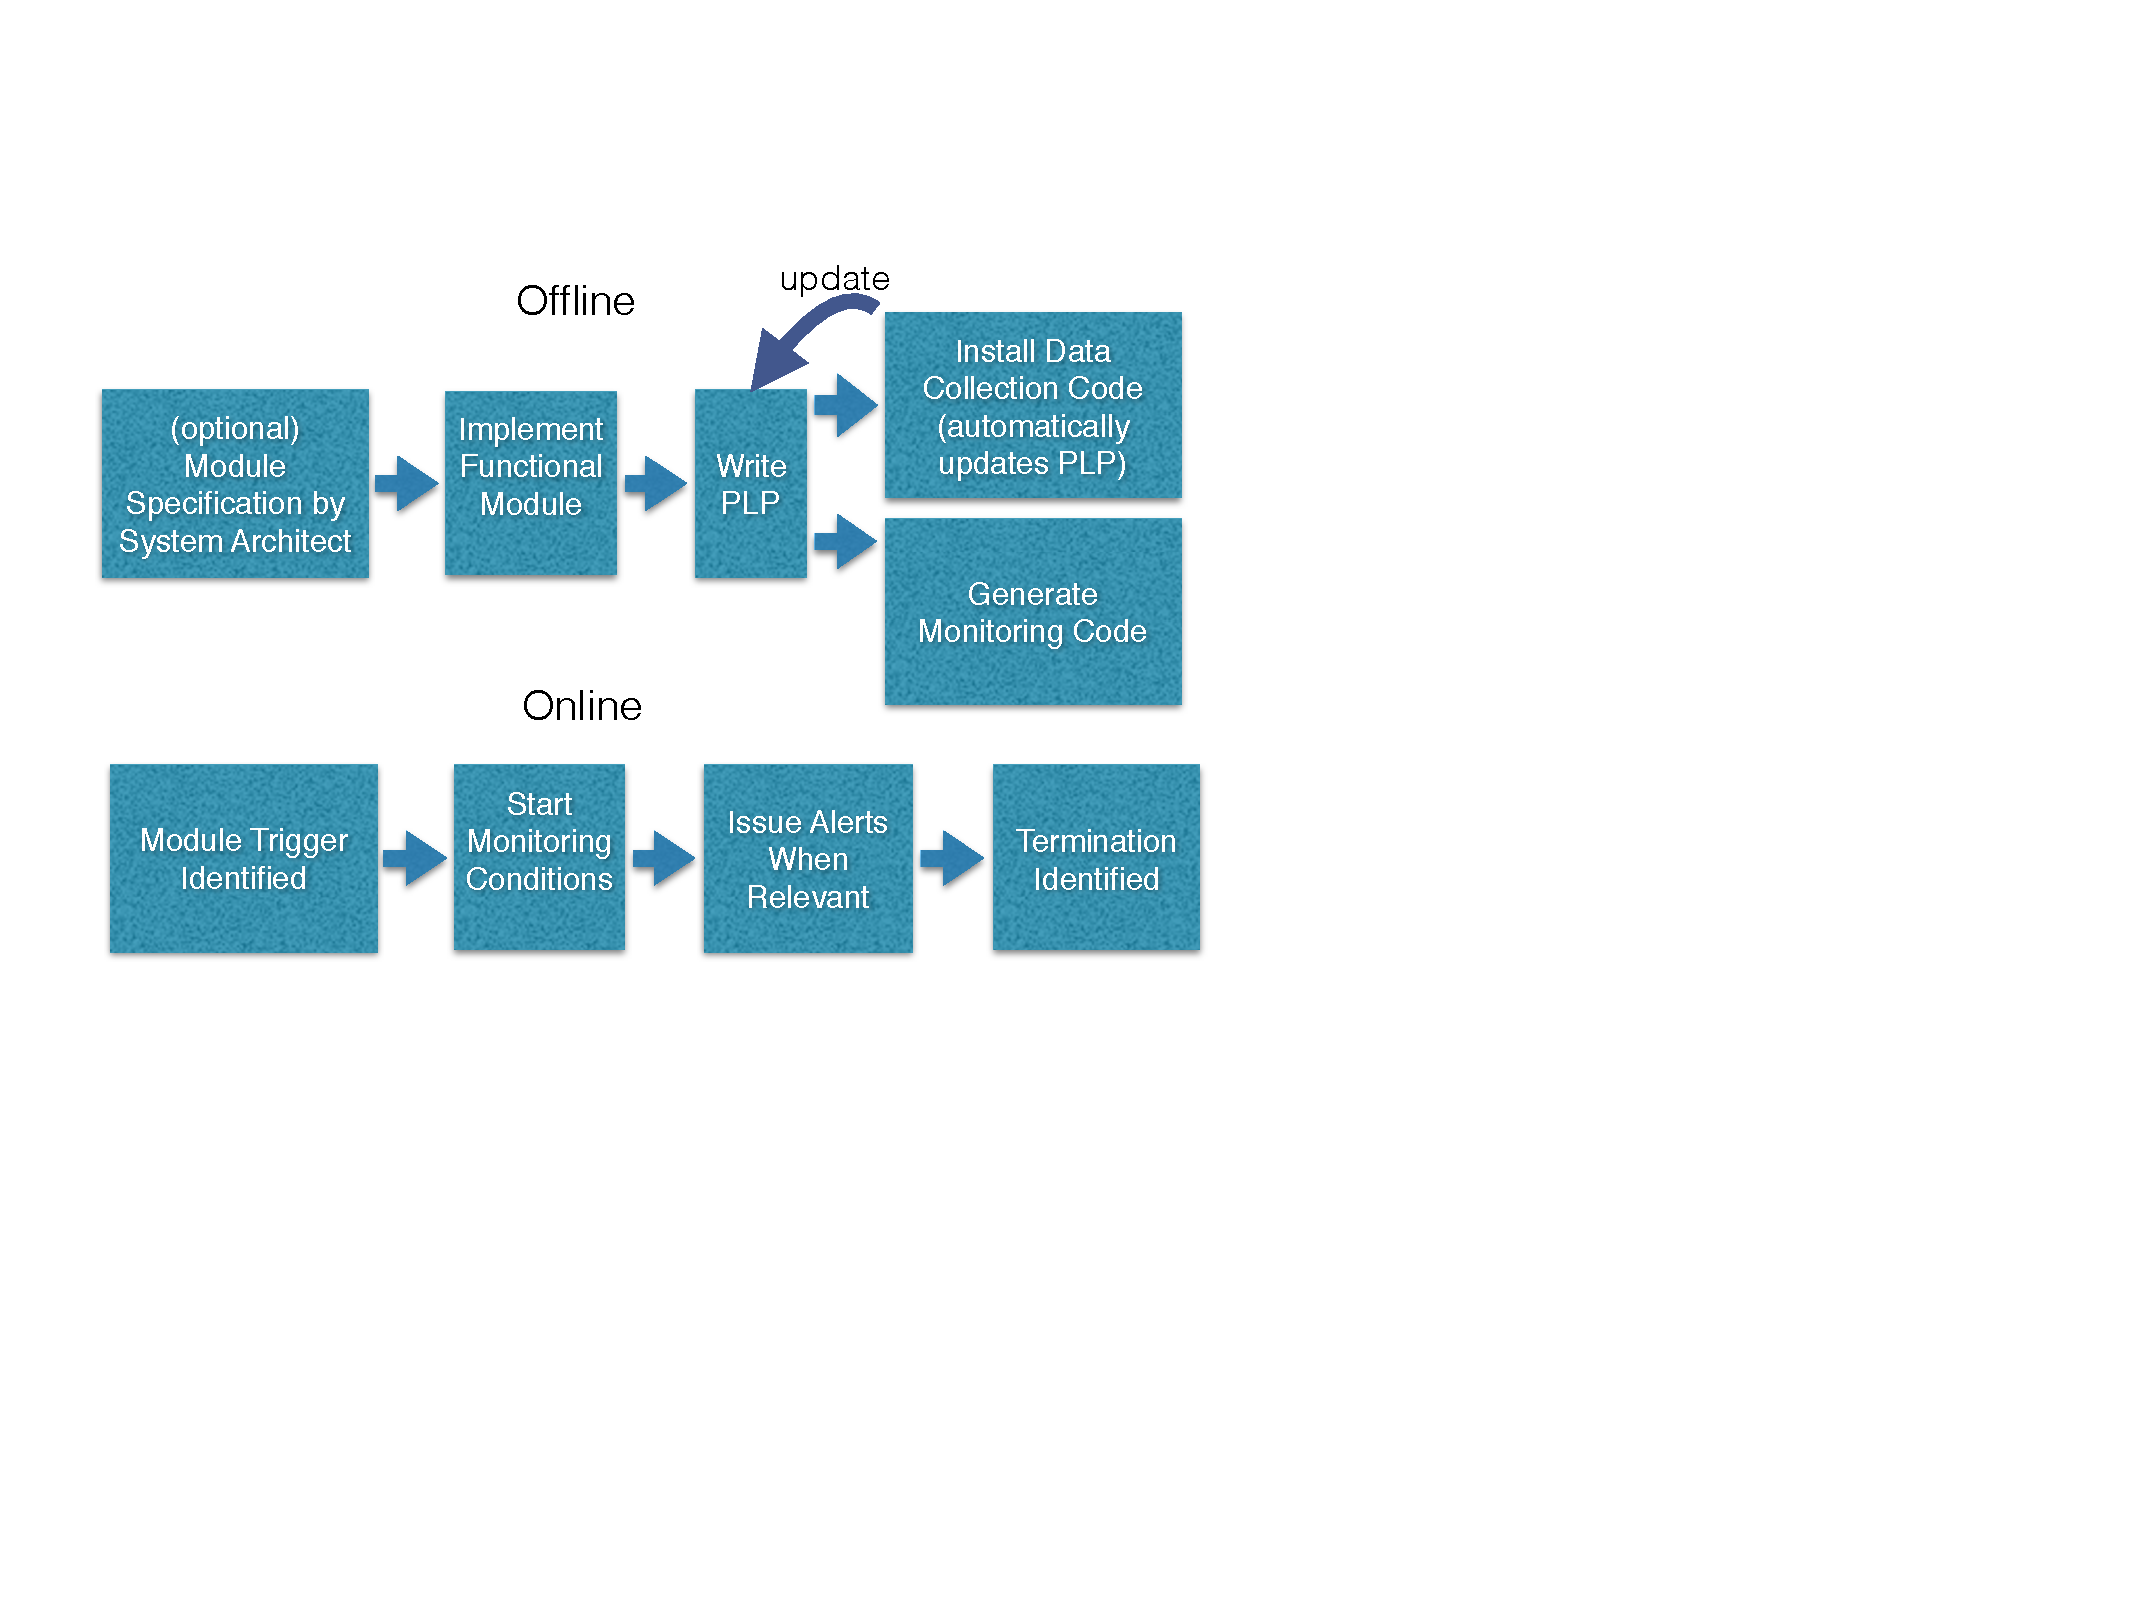
\includegraphics[scale=0.4]{methodology}
%removedVspace
\caption{Suggested Use Methodology}
\label{fig:methodology}
%removedVspace
\end{figure}

%\section{USE CASE}
Our main use case involves the use of PLPs for monitoring within the autonomous CTL, led by Israel Aerospace Industries. To date, most work done is within the Gazebo simulation environment, for which a CTL model and working environments were constructed. A PLP ROS package is installed on the real  CTL, but we do not have enough data from this installation at this point.

PLPs were used to generate monitoring
code for two modules: the way-point driver and the module that processes the IBEO laser scanner. The way-point driver has an
{\em achieve} PLP whose goal is to arrive at the next way-point (provided by the path-planner). Among some of its properties are the following two
progress conditions: the length of the planned path should decrease during an appropriate interval, and
%each the path is published by the path planning module, and
the aerial distance to the next way-point should decrease every
(different) interval.
%every time the CTL's location is published by the localization module.
During testing, the ROS node based on the way-point driver PLP helped the team find an error in the path planning module. Even though the CTL was reaching its navigation goal, the PLP node was complaining that the planned path length did not decrease. Looking into this issue, the team found that once the path planning module decided on a given path, it did not update it while the CTL was moving. Rather, it was re-publishing the same, initial path over and over again, until the CTL has reached the goal.

% Another ongoing project employing PLPs is an autonomous service robot that uses AI planning technology to respond to user requests. The  robot can perform actions like pressing an elevator button, moving between rooms, etc. For each action, a PLP is defined. Besides the benefit of automated code generation, noted earlier,
% because PLPs have precise syntax, it is easy
% to automatically compile them into planning domains in PDDL format.
% The correspondence between plan actions, PLPs, and concrete functional modules via the PDDL compiler and the glue file, makes it easy to construct a dispatcher that executes the plan on-line.
%This project demonstrates the great advantage of using PLPs: firstly, every robotic action will be monitored. This means checking for abnormalities during execution and receiveing runtime distribution and success/fail probabilities on the fly. Secondly, if ever required, statistical data gathering is supported in a convinient way. Thirdly, for this project, another tool we worked on will be used, a \emph{PDDL compiler}. The PLPs will be generated into corresponding PDDL actions which can be used to construct a plan that achieves some given goal.

%The project execution will go as follows: given PLPs for some robotic actions, corresponding PDDL actions will be generated. Those PDDL actions, and the requested goal, will be used as input for a planner. The planner will construct a plan that achieves the goal. Then, a dispatcher will be activated. The dispatcher will go action by action and trigger the corresponding robotic action (defined by a PLP). In that time, the generated monitoring code will start running and monitor the robotic action. Given a failure, replanning will be preformed.
%\maNote{I want to find a killer end phrase for this but I can't think of anything}


\begin{figure}[t]
\centering
%removedVspace
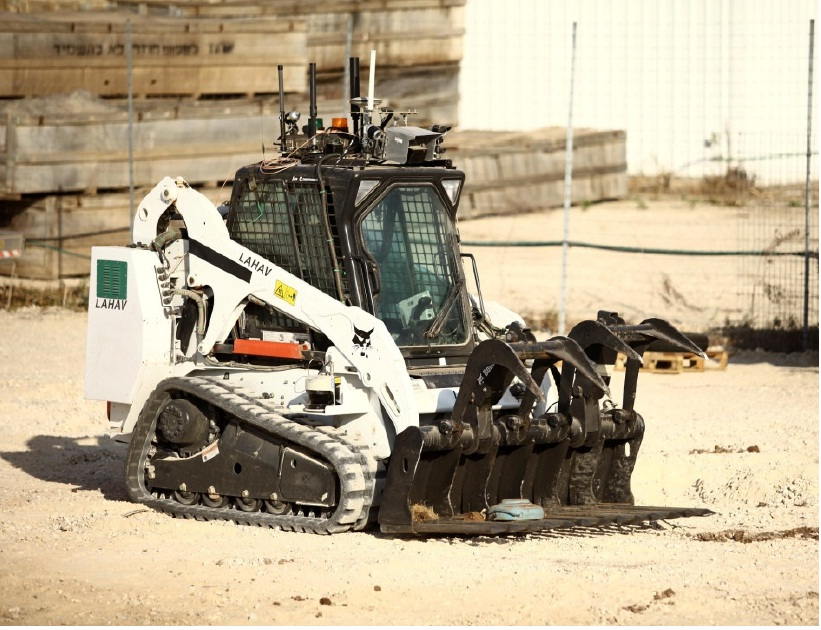
\includegraphics[scale=0.38]{bobcat1.jpg}
%removedVspace
\caption{The Autonomous CTL}
\label{fig:bobcat}
%removedVspace
\end{figure}



}


\section{Summary}
We gave an overview of formal semantics for {\em Performance Level Profiles\/} (PLPs) that maps PLPs to probabilistic timed automata. Because PLPs have a formal syntax, they are machine-readable and processable, allowing us to leverage these semantics to map actual PLPs to PTA specifications. We extended this mapping to cover compositions of PLPs within complex control structures and used UPPAAL-SMC to answer queries about plan properties.
%that use concurrency, conditions, loops, and randomization.
%This allows us to map complex scripts that invoke code fragments for which a PLP exists, into interacting PTAs. By feeding the resulting
%PTAs into a verification engine, we can  verify various properties of the script, such as the probability it will achieve certain conditions,  the probability it will maintain an invariant, and more.
Our empirical evaluation shows the potential of our approach, although
 online query evaluation is probably too slow without additional optimizations. For example, we can perform verification in parallel with plan execution.

We firmly believe that the vision of associating machine-readable documentation with code, in addition, or instead of standard natural-language documentation is realizable, especially given recent advancements in RL and natural language processing algorithms. This paper demonstrates just one of the advantages of such documentation, which
we believe can lead to far greater support for safe autonomous robots,
without requiring drastic changes in the practice of writing code.

\commentout{
Scripts are often used to combine existing capabilities to achieve more specialized or complex tasks. Verifying such scripts, built on top of such code, is challenging. PLPs


We described {\em performance level profiles\/},
a language for specifying the expected performance of functional modules. PLPs are motivated by the need to provide more precise, quantifiable,  machine-readable descriptions of module behavior. With such information, one can detect abnormal behavior, generate monitoring code automatically, and provide clear guarantees to users.
We developed a set of tools for building PLPs and using them for performance monitoring, and are currently working
on tools that automatically generate code from PLPs in support of automated planning~\citep{PlanRob16}.

%Our original motivation stems from discussions with our industry partners who lack a language and a methodology for providing their clients with reasonable performance guarantees for their products. This has led us to suggest the idea of {\em performance-level agreements} (PLA)
%a notion inspired by service-level agreements, common in telecommunications industry and in the area of web services. As robots, and especially autonomous robots operate in a much more open-ended environment, a much richer language is required for
%their formulation.

PLPs attempt to make action description language more intuitive and appropriate for robotics applications,
using well known notions of achievement and maintenance goals, analogous notions for the sensing-side of robot activity,
expected progress rates, and the {\em repeat\/} option which helps model the  notions of frequency and latency.
%commonly used by designers of robotic hardware and software.

% -- being able to provideVerification of robotic systems is an active area of research and is crucial for safe and reliable use of robots. Much of the effort in this area has been on building systems with clear guarantees that enable the generation of executable code with verified properties. Among these systems, most similar to PLPs in terms of its constructs is  PRS~\citep{PRS}, which has achieve, maintain, and observation goals, context conditions, and properties, which can mention resource consumption.
PRS is part of a large set of languages and systems for {\em building\/} robotic modules and controllers that have been developed and improved over the years. Other examples include  TCA/TDL~\citep{TCA}, RPML~\citep{RPML},  BIP~\citep{BIP2}  %~\citep{BIP,BIP2}
Genom~\citep{Genom}  or even synthesis based tools for automated controller generation, such as~\citet{KP10}.


%PLPs, on the other hand, are  descriptive rather than prescriptive and aim to aid in the use of code written in standard programming languages with standard tools. One may argue that the desirable state of affairs should be that programmers should be educated to work with formal methodologies, but this is not the current state affair, nor is it likely to be so in the near future.
%
%performance, such as success probability, expected running time, and expected progress that is missing from the above languages.
%Such descriptions can be used as a more structured, machine readable, specification language, describing the performance that the designer seeks, or as the input to automated tools that utilize information about expected behaviour for monitoring, validation, or planning. However,
%they are {\em not\/} a tool for programming robots.
%
%
Unlike these systems, PLPs are not a language or an architecture for building robots.
% -- they are not part of a complete robot architecture nor are they a language for building robots.
Their aim is to support users using existing practices
by providing them with added value services, such as monitoring code generation, planning, and plan/script verification -- the topic
of this paper. PLPs are descriptive rather than prescriptive, and for this reason, they focus on information pertaining to their module's behavior and its impact
on the system. Thus, they describe success probability, expected running time, and expected progress -- elements missing from the above languages. Of course, as the PLPs are descriptions of existing code,
the verification we provide is conditioned on the correctness of the PLP documentation for the code.
This is similar to the idea behind contracts in the Design by Contract approach~\citep{Eiffel}.
%Such descriptions can be used as a more structured, machine readable, specification language, describing the performance that the designer seeks, or as the input to automated tools that utilize information about expected behaviour for monitoring, validation, or planning, but they are {\em not\/} a tool for programming robots.
%Much like Eiffel~\citep{Eiffel}, PLPs do not enforce their "contracts".
% although monitoring them, as we suggest, is supported.
%hat is, we rely on the fact that the PLP is a faithful specification of the written code, but we cannot guarantee it.
%Instead, we offer the ability to generate code that monitors the contract, and statistics gathering tools that can, to some extent,
%verify, or improve the correctness of this specification, but only probabilistically.

%Our automated monitoring code generation is conceptually similar to
%The importance of safety monitoring for autonomous robots to their future deployment is clear to the robotics community, and several  approaches for addressing this issue have been proposed.
%run-time verification~\citep{runtimeveri} which generates code from temporal logic properties. These properties are not necessarily component centred, as in PLPs. Both are somewhat complementary to more complete, model-based pre-design techniques for defining safety constraints and interventions, such as SMOF~\citep{SMOF} and~\citep{Woodman12}, while
%is a model-based method that requires, beyond safety constraints, some sort of a model of intervention actions and a transition system. It aims to identify warning states, which are still safe, but in which some intervention is required to prevent transitions into states the violate the constraint. PLP-generated
%monitors  are based on a limited specification of components, not an entire transition system. They are passive, in the sense that they only reports on abnormal behavior, and do not provide a mechanism for interventions, yet the monitors are can be generated automatically.
%\citep{Woodman12} offer a similar methodology for safety one that starts with a hazards analysis, definition of risk requirements and constraints, identifying how the
%unsafe conditions can be avoided or reversed, and ending with a safety policy that intervenes when required. This approach is integrated into the entire design process, and is more powerful than PLP monitors. However,
%PLP-based monitoring makes post-design monitoring easy.


%The approach taken by PLPs is minimalist in the sense that it does not dictate (nor provide) particular architecture or tools for module construction. There is no doubt that tools such as BIP~\citep{BIP,BIP2} which provide a methodology for top-down construction of modules as well as tools for validating properties of the constructed system, or techniques for automated controller generation such as~\citep{KP10} provide more powerful support for the synthesis and construction of systems with guarantees.
%Nevertheless, little code is generated today using formal specification methods,
%and we expect that this state of affairs will be true in the area of robot design. On the other hand, software engineering methods are commonly used in the design of large software systems. PLPs and the provide a specification method that is similar in some ways to the commonly used SSS, yet more formal, and fits well within a methodology in which a systems engineer provides an abstract, almost textual specification, that is then implemented in code by a programmer.  They also provide a way for a designer to explain/guarantee the functional behavior of its module at some level.
%
%
%Another line in plan representation is based on the concept of reacting to
%conditions in the real world, in the form of Structured Reactive Plans (SRPs)
%\citep{Beetz00}. SRPs build upon the notion of Firby's Reactive Action Packages
%(RAPs) \citep{Firby87}, in order to create a plan-like representation of a program,
%while allowing for opportunistic actions and numerous other real-time interactions.
%SRPs also have other derivatives and applications, such as Structured Reactive Controllers (SRCs)
%\citep{Beetz99}.
%
%Although we have not closely investigated the relationship between PLPs and SRPs, several
%differences are evident.
%The way the trigger conditions for plans are expressed in SRCs looks similar
%to the way preconditions are expressed in the PLAs presented in the current paper.
%However, the semantics are different as in SRCs the action is applied as soon as the
%conditions are met, whereas in PLAs this is not implied, the effects will occur only
%{\em if} the action will occur under the given condition. That is, these notions are
%orthogonal and one might envision defining PLAs on to of SRPs as well, although we have not
%looked into how this might be done. Additionally, PLPs are designed with explicit representation of
%uncertainty, which was not a goal in SRPs, but possibly that could also be added to SRP in
%a manner similar to the way PLPs extend classical planning languages.
%

Our semantics for PLPs is obtained by mapping them to PTA. This type of semantics is sometimes called {\em translation semantics\/} and {\em semantic anchoring}.
PTAs where used for this operators with useful information about unexpected or problematic conditions, such as modules operating without the required preconditions and concurrent conditions, information about running times, and effects of modules used online. We are now working
%In addition, we have worked on the idea of automated composition of PLPs, to provide the support needs for validation and, eventually planning.

In defining PLPs we preferred intuitiveness and expressiveness over economy and succinctness. We envision that future use will lead to additional fields describing properties that are useful to know.
%being included in PLPs and see this as a plus. For example,
%we are now considering issues such as partial success capturing the idea of that some modules, in case they cannot achieve
%their desired goal, e.g., because some condition is violated, will nevertheless attempt to achieve an alternative goal, or perhaps,
%to ensure a safe end-state.
Our point is that users can always decide not to specify certain aspects of their module, and automated reasoning tools can always use only a subset of the information. For example, for generating PDDL planning domains, we use only part of information in the PLP. If a stronger planner is available, a compiler to a more informative action description language can be used, instead.
}

%In future work we aim to use PLPs to support automated planning.
%The information in them should be sufficient for a planner to select appropriate action choice and to dispatch the code modeled by the PLP during run-time. Given the mapping we described, we should be able to check the properties of synthesized controlers, and modify them.

%Thus, wee are currently working to make integration with ROSPlan~{ROSPLAN} easier and to support richer planning algorithms.


%To realize these possible benefits, the PLP definition may require farther enhancement to cover
%additional aspects of module performance.
%For example, we are now considering issues such as partial success -- e.g., sometimes a module that is unable
%to achieve its desired goal, e.g., because of some condition that is violated,
%may still be able to achieve an alternative one, or perhaps ensure some safe end-state.
%Similarly, often modules are designed with a back-up module that is called in the case of failure.
%While each such module can be specified independently, it may be desirable to have a special structure for module/backup pairs. Another possible enhancement is a more refined process model. Some modules, provide more complex services that require modeling some notion of state. Indeed, many of the formal tools developed for principled construction of robotic modules supply such a model, e.g., a state-machine~\citep{BIP2} or a Petri-Net~\citep{Montano00}.
%We wish PLPs to remain abstract specification and not nearly executable process models. Yet, the exact level of abstraction
%that will provide sufficient functionality remains an open question for future research.\\

%Finally, one important thread of current work is providing PLPs with a formal semantics by mapping them into temporal logic formulas. Ideas such as achieve, maintain, repeat, as well as frequencies, can be modeled using formulas in a suitable temporal logic. Similarly, preconditions, concurrency conditions, termination conditions etc., can also be modeled this way. Combining this information together and using a suitable theorem prover or model checker (such as PRISM~\citep{PRISM}, which support probabilistic temporal logic) can enable us to formally prove properties of a system using the PLPs of its components. Providing more added value to PLPs.\\



%\addtolength{\textheight}{-12cm}   % This command serves to balance the column lengths
                                  % on the last page of the document manually. It shortens
                                  % the textheight of the last page by a suitable amount.
                                  % This command does not take effect until the next page
                                  % so it should come on the page before the last. Make
                                  % sure that you do not shorten the textheight too much.

%%%%%%%%%%%%%%%%%%%%%%%%%%%%%%%%%%%%%%%%%%%%%%%%%%%%%%%%%%%%%%%%%%%%%%%%%%%%%%%%



%%%%%%%%%%%%%%%%%%%%%%%%%%%%%%%%%%%%%%%%%%%%%%%%%%%%%%%%%%%%%%%%%%%%%%%%%%%%%%%%



%%%%%%%%%%%%%%%%%%%%%%%%%%%%%%%%%%%%%%%%%%%%%%%%%%%%%%%%%%%%%%%%%%%%%%%%%%%%%%%%
%\section*{APPENDIX}

%Appendixes should appear before the acknowledgment.

%\section*{ACKNOWLEDGMENT}
% \section{Acknowledgements}
%  We thank the reviewers for their useful comments. This work was supported by ISF Grants 1651/19,
%  by the Israel Ministry of Science and Technology Grant 54178, and by the Lynn and William Frankel Center for Computer Science.

%%%%%%%%%%%%%%%%%%%%%%%%%%%%%%%%%%%%%%%%%%%%%%%%%%%%%%%%%%%%%%%%%%%%%%%%%%%%%%%%

\section{Acknowledgements}
This work was supported by ISF Grants 1651/19 and 1210/18, by the Israel Ministry of Science and Technology Grant 54178, and by the Lynn and William Frankel Center for Computer Science.

%\bibliographystyle{aaai}
%%\bibliographystyle{IEEEtran}
\clearpage
\bibliography{all.bib}
\end{document}


\appendix{}



\section{From Control Graph to PTA}
In this appendix we describe the mapping from control graphs to PTAs and discuss some limitations imposed on our models due to UPPAAL's expressive power.

The mapping works by converting each node to a PTA and connecting them. We now describe the conversion of each node.
In the following PTA\textsubscript{Node} templates, PTAs\textsubscript{Node} starts at \textit{``init\_node"}. To proceed, either all (``OP" is logical AND) immediate predecessors, or any ("OP" is logical OR) immediate predecessor, need to finish.
\subsection{PTA\textsubscript{PLP} launcher node}
\frameImage{nodeSequential.eps}{3.3in}{1.62in}{Template for PTA\textsubscript{Node} launcher of PTAs\textsubscript{PLP}}

When the condition to run (the condition that
appears between \textit{"init\_node"} and \textit{"wait"}) is satisfied, the PTA\textsubscript{Node} goes over the sequence of PTAs\textsubscript{PLP} it should execute, and signals to each PTA\textsubscript{PLP} in its time, to run, using the \textit{"pta\_start[i]"} ($\forall i \in \big[1..m\big]$) channel. It then waits for PTA\textsubscript{PLP} to complete running on \textit{"pta\_done[i]"} channel. When all PTAs\textsubscript{PLP} finished running, PTA\textsubscript{Node} updates \textit{"successor\_can\_run"} so that the successor PTA\textsubscript{Node} can run. Eventually, it signals to successor PTA\textsubscript{Node} on \textit{"try\_to\_run\_successor"} channel to start running if possible.

\subsection{Probabilistic node}
\frameImage{nodeProbability.eps}{3.3in}{2.9in}{Template for probabilistic PTA\textsubscript{Node}}
\par When the condition to run is satisfied, the PTA\textsubscript{Node} waits in a \textit{"wait"} state, for a time interval determined by the control graph. Then the PTA\textsubscript{Node} probabilistically chooses a single path to follow, out of the possible $k$ paths, according to the probability of each path. Then, the PTA\textsubscript{Node} updates a designated flag \textit{"successor\_can\_run[i]"} ($i \in \big[1..k\big]$) for a successor node, to let the successor know when to run. Eventually, PTA\textsubscript{Node} signals to the successor on a\textit{"try\_to\_run\_successor[i]"} channel, to check if it can start.%
\footnote{We need both a flag and a signal along a channel in case there are more than one predecessor.}
%\rNote{Why do you need both a flag and a signal?}
%\aNote{Nodes with a single immediate predecessor can be forced to run either with a flag (guard+invariant) or signal. But nodes that need two or more immediate predecessor, have to remember which predecessors are done, but they can't run until the last immediate predecessor is done. If we use only flags (with invariants) without a signal, the node would not be compelled to run immediately. If we use only signals, we would not remember who is done.  }
\subsection{Conditional node}
\frameImage{nodeCondition.eps}{3.3in}{2.9in}{Template for conditional PTA\textsubscript{Node}}

When the condition to run is satisfied, the PTA\textsubscript{Node} waits in a \textit{"wait"} state, for a time interval determined by the control graph. In the PTA\textsubscript{Node} template above there are $k$ conditions:\textit{"condition[1] == true, …, condition[k] == true"}, used as place holders.
Real conditions may be more complex. The PTA evaluates the conditions and chooses a single satisfied condition non-deterministically.
%, to follow its running path.
Afterwards, PTA\textsubscript{Node} updates a designated flag \textit{"successor\_can\_run[i]"} ($i \in \big[1..k\big]$) for a successor node, to let the successor know when to run. Eventually, PTA\textsubscript{Node} signals to the successor on a\textit{"try\_to\_run\_successor[i]"} channel, to check if it can start.


\subsection{Concurrent node}
\frameImage{nodeConcurrent.eps}{3.5in}{1.52in}{Template for concurrent node}

%\rNote{again what does the condition to run mean}
%\aNote{It's the condition between \textit{"init\_node"} and \textit{"wait"}, that allows for current node to run, according to immediate predecessors completion status. "OP" can be AND or OR: AND -- to wait for all immediate predecessors to end. OR -- to wait that for even one immediate predecessors to end.}
When the condition to run is satisfied, PTA\textsubscript{Node} waits in a \textit{"wait"} state for a time interval determined by the control graph. Then, the PTA\textsubscript{Node} updates \textit{"successor\_can\_run[i]"} ($\forall i \in \big[1..k\big]$) for all successors nodes. Then, the PTA\textsubscript{Node} signals to each successor on the \textit{"try\_to\_run\_successor[i]" }channel to check if it can run.
%\rNote{Is there a reason it cannot run?}
%\aNote{If it needs other nodes to end -- in case of "*" = "AND" with two or more immediate predecessors.}
Notice that other nodes receive the signal on \textit{"try\_to\_run\_successor[i]"} channel in a sequential manner. If their run condition is fulfilled and they can run, they will only pass the synchronization edge. Other internal transitions for every successor are not restricted by the initial order, and they can happen concurrently. For example, if node \textit{"id\textsubscript{1}"} passed synchronization first, and then node \textit{"id\textsubscript{2}"}, the very next transition can belong to either \textit{"id\textsubscript{2}"} or \textit{"id\textsubscript{1}"}, and each execution can produce different combination of transition events.%
\footnote{This is the well known interleaving semantics of concurrent processes, which we assume to be valid as
long as the concurrency conditions of each PLP are satisfied.
}
%\rNote{This is not clear to me. I thought that the nodes are run concurrently. So what is the meaning of a different schedule?}
%\aNote{Conceptually PTAs run in a concurrent manner, but practically they are cartesian product of PTAs, and there is always an order between any two transitions, even those that appear to happen at the same time. Here I want to explain that although I call successor nodes sequentially, the meaningful part of their internal transitions can happen out of the initial order, conceptually parallelly.}
%\rNote{As far as I know, in principle, it is possible to define a cartersian product over the action space, in which case you can model true concurrency. However, I imagine this is not what UPPAAL does.}
%\aNote{I'm not sure about that.}
%\listoftodos{}

\subsection{Limitations}
There are a few restrictions in UPPAAL that require a slight adaptation to the PTAs defined. Variables in UPPAAL are restricted to integer values. To minimize loss of precision we multiply all the variables and durations by an adjustable precision factor and truncate the fractional part.
\par Integers in UPPAAL range from -32768 to 32767. Because we rely on integers for clocks and variables, we are limited to values in this range. The precision factor, which is larger than 1, reduces the time intervals and variables we can simulate and verify even further. Therefore it is important to notice that with a precision factor of $X$, we are limited by variables in the range $\left [ - \frac{32,768}{X}, \frac{32,767}{X} \right ]$. Clock values can range up to $\frac{1,073,741,822}{X}$ time units.
\par UPPAAL supports uniform and exponential distributions but not general run time distributions. To implement other distributions, we create an approximation with uniform distribution by discretizing the original distribution.
\par Invariants in UPPAAL are restricted to conjunction/disjunction of simple comparisons between variables/clocks and constant values. Due to the heavy reliance on invariants in the PTAs\textsubscript{PLP}, we made a few changes  to PTAs\textsubscript{PLP} to work around this problem. We need to be able to make immediate transitions when a value of a variable in a critical condition changes. This can be achieved by sending a signal on a channel for each changed variable. Therefore, critical conditions that contain a few variables should have an edge with a channel corresponding to every variable, and guard condition equal to the original condition. This forces us to make sure that any write to a variable that may be part of a critical condition will also send a signal on a channel corresponding to that variable. This issue was addressed  by creating a mechanism to read/write shared variables by any PTA, and with channels to signal about the change to other PTAs without additional time delays to the process.
Additional details can be found in~\citet{kovalchu2018}.


\end{document}